\documentclass[1p]{elsarticle_modified}
%\bibliographystyle{elsarticle-num}

%\usepackage[colorlinks]{hyperref}
%\usepackage{abbrmath_seonhwa} %\Abb, \Ascr, \Acal ,\Abf, \Afrak
\usepackage{amsfonts}
\usepackage{amssymb}
\usepackage{amsmath}
\usepackage{amsthm}
\usepackage{scalefnt}
\usepackage{amsbsy}
\usepackage{kotex}
\usepackage{caption}
\usepackage{subfig}
\usepackage{color}
\usepackage{graphicx}
\usepackage{xcolor} %% white, black, red, green, blue, cyan, magenta, yellow
\usepackage{float}
\usepackage{setspace}
\usepackage{hyperref}

\usepackage{tikz}
\usetikzlibrary{arrows}

\usepackage{multirow}
\usepackage{array} % fixed length table
\usepackage{hhline}

%%%%%%%%%%%%%%%%%%%%%
\makeatletter
\renewcommand*\env@matrix[1][\arraystretch]{%
	\edef\arraystretch{#1}%
	\hskip -\arraycolsep
	\let\@ifnextchar\new@ifnextchar
	\array{*\c@MaxMatrixCols c}}
\makeatother %https://tex.stackexchange.com/questions/14071/how-can-i-increase-the-line-spacing-in-a-matrix
%%%%%%%%%%%%%%%

\usepackage[normalem]{ulem}

\newcommand{\msout}[1]{\ifmmode\text{\sout{\ensuremath{#1}}}\else\sout{#1}\fi}
%SOURCE: \msout is \stkout macro in https://tex.stackexchange.com/questions/20609/strikeout-in-math-mode

\newcommand{\cancel}[1]{
	\ifmmode
	{\color{red}\msout{#1}}
	\else
	{\color{red}\sout{#1}}
	\fi
}

\newcommand{\add}[1]{
	{\color{blue}\uwave{#1}}
}

\newcommand{\replace}[2]{
	\ifmmode
	{\color{red}\msout{#1}}{\color{blue}\uwave{#2}}
	\else
	{\color{red}\sout{#1}}{\color{blue}\uwave{#2}}
	\fi
}

\newcommand{\Sol}{\mathcal{S}} %segment
\newcommand{\D}{D} %diagram
\newcommand{\A}{\mathcal{A}} %arc


%%%%%%%%%%%%%%%%%%%%%%%%%%%%%5 test

\def\sl{\operatorname{\textup{SL}}(2,\Cbb)}
\def\psl{\operatorname{\textup{PSL}}(2,\Cbb)}
\def\quan{\mkern 1mu \triangleright \mkern 1mu}

\theoremstyle{definition}
\newtheorem{thm}{Theorem}[section]
\newtheorem{prop}[thm]{Proposition}
\newtheorem{lem}[thm]{Lemma}
\newtheorem{ques}[thm]{Question}
\newtheorem{cor}[thm]{Corollary}
\newtheorem{defn}[thm]{Definition}
\newtheorem{exam}[thm]{Example}
\newtheorem{rmk}[thm]{Remark}
\newtheorem{alg}[thm]{Algorithm}

\newcommand{\I}{\sqrt{-1}}
\begin{document}

%\begin{frontmatter}
%
%\title{Boundary parabolic representations of knots up to 8 crossings}
%
%%% Group authors per affiliation:
%\author{Yunhi Cho} 
%\address{Department of Mathematics, University of Seoul, Seoul, Korea}
%\ead{yhcho@uos.ac.kr}
%
%
%\author{Seonhwa Kim} %\fnref{s_kim}}
%\address{Center for Geometry and Physics, Institute for Basic Science, Pohang, 37673, Korea}
%\ead{ryeona17@ibs.re.kr}
%
%\author{Hyuk Kim}
%\address{Department of Mathematical Sciences, Seoul National University, Seoul 08826, Korea}
%\ead{hyukkim@snu.ac.kr}
%
%\author{Seokbeom Yoon}
%\address{Department of Mathematical Sciences, Seoul National University, Seoul, 08826,  Korea}
%\ead{sbyoon15@snu.ac.kr}
%
%\begin{abstract}
%We find all boundary parabolic representation of knots up to 8 crossings.
%
%\end{abstract}
%\begin{keyword}
%    \MSC[2010] 57M25 
%\end{keyword}
%
%\end{frontmatter}

%\linenumbers
%\tableofcontents
%
\newcommand\colored[1]{\textcolor{white}{\rule[-0.35ex]{0.8em}{1.4ex}}\kern-0.8em\color{red} #1}%
%\newcommand\colored[1]{\textcolor{white}{ #1}\kern-2.17ex	\textcolor{white}{ #1}\kern-1.81ex	\textcolor{white}{ #1}\kern-2.15ex\color{red}#1	}

{\Large $\underline{12a_{0030}~(K12a_{0030})}$}

\setlength{\tabcolsep}{10pt}
\renewcommand{\arraystretch}{1.6}
\vspace{1cm}\begin{tabular}{m{100pt}>{\centering\arraybackslash}m{274pt}}
\multirow{5}{120pt}{
	\centering
	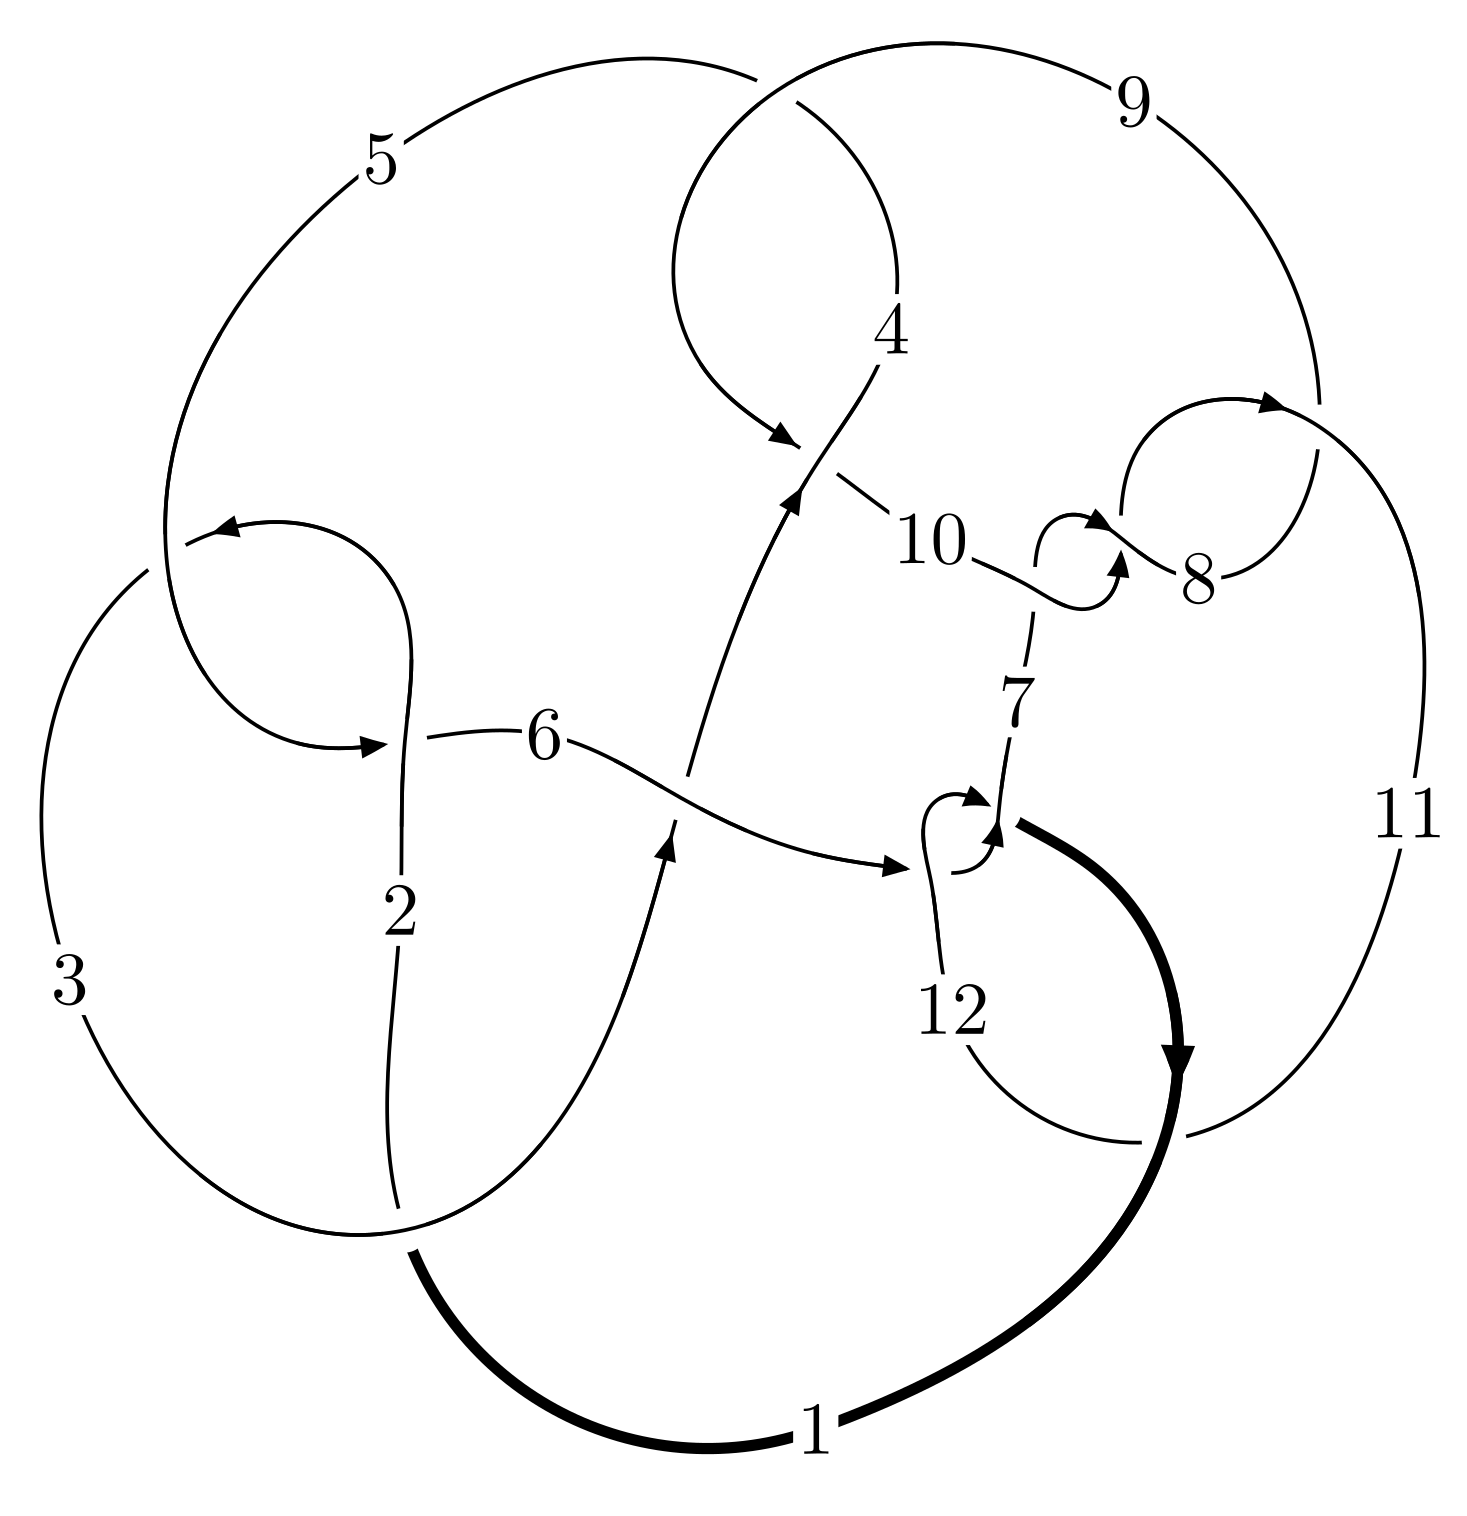
\includegraphics[width=112pt]{../../../GIT/diagram.site/Diagrams/png/831_12a_0030.png}\\
\ \ \ A knot diagram\footnotemark}&
\allowdisplaybreaks
\textbf{Linearized knot diagam} \\
\cline{2-2}
 &
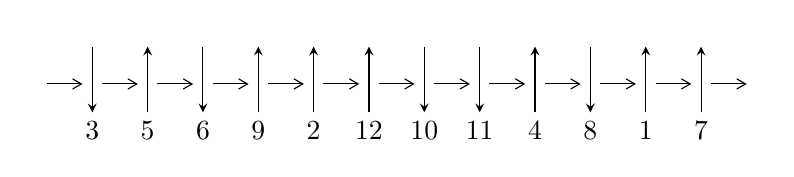
\begin{tikzpicture}[x=20pt, y=17pt]
	% nodes
	\node (C0) at (0, 0) {};
	\node (C1) at (1, 0) {};
	\node (C1U) at (1, +1) {};
	\node (C1D) at (1, -1) {3};

	\node (C2) at (2, 0) {};
	\node (C2U) at (2, +1) {};
	\node (C2D) at (2, -1) {5};

	\node (C3) at (3, 0) {};
	\node (C3U) at (3, +1) {};
	\node (C3D) at (3, -1) {6};

	\node (C4) at (4, 0) {};
	\node (C4U) at (4, +1) {};
	\node (C4D) at (4, -1) {9};

	\node (C5) at (5, 0) {};
	\node (C5U) at (5, +1) {};
	\node (C5D) at (5, -1) {2};

	\node (C6) at (6, 0) {};
	\node (C6U) at (6, +1) {};
	\node (C6D) at (6, -1) {12};

	\node (C7) at (7, 0) {};
	\node (C7U) at (7, +1) {};
	\node (C7D) at (7, -1) {10};

	\node (C8) at (8, 0) {};
	\node (C8U) at (8, +1) {};
	\node (C8D) at (8, -1) {11};

	\node (C9) at (9, 0) {};
	\node (C9U) at (9, +1) {};
	\node (C9D) at (9, -1) {4};

	\node (C10) at (10, 0) {};
	\node (C10U) at (10, +1) {};
	\node (C10D) at (10, -1) {8};

	\node (C11) at (11, 0) {};
	\node (C11U) at (11, +1) {};
	\node (C11D) at (11, -1) {1};

	\node (C12) at (12, 0) {};
	\node (C12U) at (12, +1) {};
	\node (C12D) at (12, -1) {7};
	\node (C13) at (13, 0) {};

	% arrows
	\draw[->,>={angle 60}]
	(C0) edge (C1) (C1) edge (C2) (C2) edge (C3) (C3) edge (C4) (C4) edge (C5) (C5) edge (C6) (C6) edge (C7) (C7) edge (C8) (C8) edge (C9) (C9) edge (C10) (C10) edge (C11) (C11) edge (C12) (C12) edge (C13) ;	\draw[->,>=stealth]
	(C1U) edge (C1D) (C2D) edge (C2U) (C3U) edge (C3D) (C4D) edge (C4U) (C5D) edge (C5U) (C6D) edge (C6U) (C7U) edge (C7D) (C8U) edge (C8D) (C9D) edge (C9U) (C10U) edge (C10D) (C11D) edge (C11U) (C12D) edge (C12U) ;
	\end{tikzpicture} \\
\hhline{~~} \\& 
\textbf{Solving Sequence} \\ \cline{2-2} 
 &
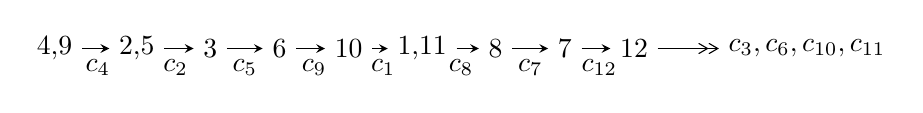
\begin{tikzpicture}[x=25pt, y=7pt]
	% node
	\node (A0) at (-1/8, 0) {4,9};
	\node (A1) at (17/16, 0) {2,5};
	\node (A2) at (17/8, 0) {3};
	\node (A3) at (25/8, 0) {6};
	\node (A4) at (33/8, 0) {10};
	\node (A5) at (83/16, 0) {1,11};
	\node (A6) at (25/4, 0) {8};
	\node (A7) at (29/4, 0) {7};
	\node (A8) at (33/4, 0) {12};
	\node (C1) at (1/2, -1) {$c_{4}$};
	\node (C2) at (13/8, -1) {$c_{2}$};
	\node (C3) at (21/8, -1) {$c_{5}$};
	\node (C4) at (29/8, -1) {$c_{9}$};
	\node (C5) at (37/8, -1) {$c_{1}$};
	\node (C6) at (23/4, -1) {$c_{8}$};
	\node (C7) at (27/4, -1) {$c_{7}$};
	\node (C8) at (31/4, -1) {$c_{12}$};
	\node (A9) at (43/4, 0) {$c_{3},c_{6},c_{10},c_{11}$};

	% edge
	\draw[->,>=stealth]	
	(A0) edge (A1) (A1) edge (A2) (A2) edge (A3) (A3) edge (A4) (A4) edge (A5) (A5) edge (A6) (A6) edge (A7) (A7) edge (A8) ;
	\draw[->>,>={angle 60}]	
	(A8) edge (A9);
\end{tikzpicture} \\ 

\end{tabular} \\

\footnotetext{
The image of knot diagram is generated by the software ``\textbf{Draw programme}" developed by Andrew Bartholomew(\url{http://www.layer8.co.uk/maths/draw/index.htm\#Running-draw}), where we modified some parts for our purpose(\url{https://github.com/CATsTAILs/LinksPainter}).
}\phantom \\ \newline 
\centering \textbf{Ideals for irreducible components\footnotemark of $X_{\text{par}}$} 
 
\begin{align*}
I^u_{1}&=\langle 
2.97380\times10^{162} u^{76}-7.99163\times10^{162} u^{75}+\cdots+1.45795\times10^{166} d-5.67098\times10^{165},\\
\phantom{I^u_{1}}&\phantom{= \langle  }4.24191\times10^{162} u^{76}-1.61625\times10^{163} u^{75}+\cdots+1.45795\times10^{166} c+2.78196\times10^{165},\\
\phantom{I^u_{1}}&\phantom{= \langle  }6.76436\times10^{182} u^{76}-1.29212\times10^{183} u^{75}+\cdots+1.08760\times10^{185} b-1.19824\times10^{185},\\
\phantom{I^u_{1}}&\phantom{= \langle  }1.65541\times10^{183} u^{76}-4.27644\times10^{183} u^{75}+\cdots+2.17520\times10^{185} a+1.69038\times10^{186},\\
\phantom{I^u_{1}}&\phantom{= \langle  }u^{77}-2 u^{76}+\cdots-2560 u^2-512\rangle \\
I^u_{2}&=\langle 
- c^2 u+d- c,\;u^3 c+c^3+u^2 c- u^3+c u- u+1,\;- u^2+b+u-1,\;u^3- u^2+a+u-1,\;u^4+u^2- u+1\rangle \\
I^u_{3}&=\langle 
- c^2 u+d- c,\;-2 u^5 c- u^4 c- u^5-3 u^3 c- u^4+c^3-2 u^2 c-2 u^3-2 c u-2 u^2-2 c-2 u-2,\\
\phantom{I^u_{3}}&\phantom{= \langle  }-2 u^5- u^4-3 u^3-2 u^2+b-3 u-2,\;- u^4- u^2+a- u-1,\;u^6+u^5+2 u^4+2 u^3+2 u^2+2 u+1\rangle \\
\\
I^v_{1}&=\langle 
a,\;d,\;c- v,\;b- v,\;v^2- v+1\rangle \\
I^v_{2}&=\langle 
a,\;d+v+1,\;a v+c+1,\;b+v,\;v^2+v+1\rangle \\
I^v_{3}&=\langle 
c,\;d-1,\;b,\;a-1,\;v-1\rangle \\
I^v_{4}&=\langle 
a,\;d b+d a- c b- d+b-1,\;a^2 d- c b a- d a+c b+b a+d- c- a+1,\;d v-1,\;c v+b a- b v- b- a,\\
\phantom{I^v_{4}}&\phantom{= \langle  }b^2- b+1\rangle \\
\end{align*}
\raggedright * 6 irreducible components of $\dim_{\mathbb{C}}=0$, with total 112 representations.\\
\raggedright * 1 irreducible components of $\dim_{\mathbb{C}}=1$ \\
\footnotetext{All coefficients of polynomials are rational numbers. But the coefficients are sometimes approximated in decimal forms when there is not enough margin.}
\newpage
\renewcommand{\arraystretch}{1}
\centering \section*{I. $I^u_{1}= \langle 2.97\times10^{162} u^{76}-7.99\times10^{162} u^{75}+\cdots+1.46\times10^{166} d-5.67\times10^{165},\;4.24\times10^{162} u^{76}-1.62\times10^{163} u^{75}+\cdots+1.46\times10^{166} c+2.78\times10^{165},\;6.76\times10^{182} u^{76}-1.29\times10^{183} u^{75}+\cdots+1.09\times10^{185} b-1.20\times10^{185},\;1.66\times10^{183} u^{76}-4.28\times10^{183} u^{75}+\cdots+2.18\times10^{185} a+1.69\times10^{186},\;u^{77}-2 u^{76}+\cdots-2560 u^2-512 \rangle$}
\flushleft \textbf{(i) Arc colorings}\\
\begin{tabular}{m{7pt} m{180pt} m{7pt} m{180pt} }
\flushright $a_{4}=$&$\begin{pmatrix}1\\0\end{pmatrix}$ \\
\flushright $a_{9}=$&$\begin{pmatrix}0\\u\end{pmatrix}$ \\
\flushright $a_{2}=$&$\begin{pmatrix}-0.00761038 u^{76}+0.0196600 u^{75}+\cdots+4.69111 u-7.77114\\-0.00621954 u^{76}+0.0118805 u^{75}+\cdots+6.90325 u+1.10173\end{pmatrix}$ \\
\flushright $a_{5}=$&$\begin{pmatrix}1\\- u^2\end{pmatrix}$ \\
\flushright $a_{3}=$&$\begin{pmatrix}-0.00903125 u^{76}+0.0210962 u^{75}+\cdots+7.69784 u-4.39652\\-0.00575546 u^{76}+0.0105565 u^{75}+\cdots+7.63073 u+1.82138\end{pmatrix}$ \\
\flushright $a_{6}=$&$\begin{pmatrix}-0.0108390 u^{76}+0.0188168 u^{75}+\cdots+14.5481 u-0.522142\\0.00170046 u^{76}-0.00573767 u^{75}+\cdots-1.46268 u+2.50020\end{pmatrix}$ \\
\flushright $a_{10}=$&$\begin{pmatrix}u\\u\end{pmatrix}$ \\
\flushright $a_{1}=$&$\begin{pmatrix}-0.0125394 u^{76}+0.0245545 u^{75}+\cdots+16.0108 u-3.02234\\-0.00622485 u^{76}+0.0135037 u^{75}+\cdots+7.88286 u-2.23172\end{pmatrix}$ \\
\flushright $a_{11}=$&$\begin{pmatrix}-0.000290951 u^{76}+0.00110858 u^{75}+\cdots+1.36870 u-0.190813\\-0.000203972 u^{76}+0.000548142 u^{75}+\cdots+0.515526 u+0.388970\end{pmatrix}$ \\
\flushright $a_{8}=$&$\begin{pmatrix}0.0000869789 u^{76}-0.000560439 u^{75}+\cdots-0.853173 u+0.579783\\-0.000203972 u^{76}+0.000548142 u^{75}+\cdots+0.515526 u+0.388970\end{pmatrix}$ \\
\flushright $a_{7}=$&$\begin{pmatrix}-0.000208604 u^{76}-0.0000329385 u^{75}+\cdots-1.00214 u+0.849444\\-0.000499554 u^{76}+0.00107564 u^{75}+\cdots+0.366559 u+0.658630\end{pmatrix}$ \\
\flushright $a_{12}=$&$\begin{pmatrix}-0.0150036 u^{76}+0.0284788 u^{75}+\cdots+20.0911 u-2.34221\\-0.00485367 u^{76}+0.0102965 u^{75}+\cdots+6.71768 u-1.05079\end{pmatrix}$\\&\end{tabular}
\flushleft \textbf{(ii) Obstruction class $= -1$}\\~\\
\flushleft \textbf{(iii) Cusp Shapes $= 0.0221138 u^{76}-0.0478032 u^{75}+\cdots-21.6023 u-0.388088$}\\~\\
\newpage\renewcommand{\arraystretch}{1}
\flushleft \textbf{(iv) u-Polynomials at the component}\newline \\
\begin{tabular}{m{50pt}|m{274pt}}
Crossings & \hspace{64pt}u-Polynomials at each crossing \\
\hline $$\begin{aligned}c_{1}\end{aligned}$$&$\begin{aligned}
&u^{77}+36 u^{76}+\cdots+216 u-16
\end{aligned}$\\
\hline $$\begin{aligned}c_{2},c_{5}\end{aligned}$$&$\begin{aligned}
&u^{77}+2 u^{76}+\cdots+27 u^2-4
\end{aligned}$\\
\hline $$\begin{aligned}c_{3}\end{aligned}$$&$\begin{aligned}
&u^{77}-2 u^{76}+\cdots+351912 u-66564
\end{aligned}$\\
\hline $$\begin{aligned}c_{4},c_{9}\end{aligned}$$&$\begin{aligned}
&u^{77}-2 u^{76}+\cdots-2560 u^2-512
\end{aligned}$\\
\hline $$\begin{aligned}c_{6},c_{12}\end{aligned}$$&$\begin{aligned}
&u^{77}+8 u^{76}+\cdots-72 u-16
\end{aligned}$\\
\hline $$\begin{aligned}c_{7},c_{8},c_{10}\end{aligned}$$&$\begin{aligned}
&u^{77}-8 u^{76}+\cdots-72 u-16
\end{aligned}$\\
\hline $$\begin{aligned}c_{11}\end{aligned}$$&$\begin{aligned}
&u^{77}-34 u^{76}+\cdots+1568 u-256
\end{aligned}$\\
\hline
\end{tabular}\\~\\
\newpage\renewcommand{\arraystretch}{1}
\flushleft \textbf{(v) Riley Polynomials at the component}\newline \\
\begin{tabular}{m{50pt}|m{274pt}}
Crossings & \hspace{64pt}Riley Polynomials at each crossing \\
\hline $$\begin{aligned}c_{1}\end{aligned}$$&$\begin{aligned}
&y^{77}+12 y^{76}+\cdots+84256 y-256
\end{aligned}$\\
\hline $$\begin{aligned}c_{2},c_{5}\end{aligned}$$&$\begin{aligned}
&y^{77}+36 y^{76}+\cdots+216 y-16
\end{aligned}$\\
\hline $$\begin{aligned}c_{3}\end{aligned}$$&$\begin{aligned}
&y^{77}-12 y^{76}+\cdots+120020616504 y-4430766096
\end{aligned}$\\
\hline $$\begin{aligned}c_{4},c_{9}\end{aligned}$$&$\begin{aligned}
&y^{77}+30 y^{76}+\cdots-2621440 y-262144
\end{aligned}$\\
\hline $$\begin{aligned}c_{6},c_{12}\end{aligned}$$&$\begin{aligned}
&y^{77}-34 y^{76}+\cdots+1568 y-256
\end{aligned}$\\
\hline $$\begin{aligned}c_{7},c_{8},c_{10}\end{aligned}$$&$\begin{aligned}
&y^{77}-74 y^{76}+\cdots+7712 y-256
\end{aligned}$\\
\hline $$\begin{aligned}c_{11}\end{aligned}$$&$\begin{aligned}
&y^{77}+26 y^{76}+\cdots+3416576 y-65536
\end{aligned}$\\
\hline
\end{tabular}\\~\\
\newpage\flushleft \textbf{(vi) Complex Volumes and Cusp Shapes}
$$\begin{array}{c|c|c}  
\text{Solutions to }I^u_{1}& \I (\text{vol} + \sqrt{-1}CS) & \text{Cusp shape}\\
 \hline 
\begin{aligned}
u &= \phantom{-}0.508886 + 0.845592 I \\
a &= -2.01821 + 2.48278 I \\
b &= \phantom{-}0.67033 + 1.82257 I \\
c &= \phantom{-}0.464983 + 0.518986 I \\
d &= \phantom{-}0.029827 + 0.719662 I\end{aligned}
 & \phantom{-}2.40889 + 4.27390 I & \phantom{-}3.74115 - 6.44221 I \\ \hline\begin{aligned}
u &= \phantom{-}0.508886 - 0.845592 I \\
a &= -2.01821 - 2.48278 I \\
b &= \phantom{-}0.67033 - 1.82257 I \\
c &= \phantom{-}0.464983 - 0.518986 I \\
d &= \phantom{-}0.029827 - 0.719662 I\end{aligned}
 & \phantom{-}2.40889 - 4.27390 I & \phantom{-}3.74115 + 6.44221 I \\ \hline\begin{aligned}
u &= -0.848496 + 0.585068 I \\
a &= \phantom{-}0.774643 + 0.166861 I \\
b &= \phantom{-}0.208609 + 0.303408 I \\
c &= -0.508850 + 0.474076 I \\
d &= -0.255576 + 0.903445 I\end{aligned}
 & \phantom{-}3.78378 + 2.11500 I & \phantom{-}7.65464 - 1.99007 I \\ \hline\begin{aligned}
u &= -0.848496 - 0.585068 I \\
a &= \phantom{-}0.774643 - 0.166861 I \\
b &= \phantom{-}0.208609 - 0.303408 I \\
c &= -0.508850 - 0.474076 I \\
d &= -0.255576 - 0.903445 I\end{aligned}
 & \phantom{-}3.78378 - 2.11500 I & \phantom{-}7.65464 + 1.99007 I \\ \hline\begin{aligned}
u &= -0.990280 + 0.319237 I \\
a &= \phantom{-}0.787830 + 0.083627 I \\
b &= -0.082157 + 0.217726 I \\
c &= \phantom{-}1.249660 + 0.250247 I \\
d &= -0.434460 + 0.109424 I\end{aligned}
 & -2.98745 + 0.86657 I & \phantom{-0.000000 } 0 \\ \hline\begin{aligned}
u &= -0.990280 - 0.319237 I \\
a &= \phantom{-}0.787830 - 0.083627 I \\
b &= -0.082157 - 0.217726 I \\
c &= \phantom{-}1.249660 - 0.250247 I \\
d &= -0.434460 - 0.109424 I\end{aligned}
 & -2.98745 - 0.86657 I & \phantom{-0.000000 } 0\\
 \hline 
 \end{array}$$\newpage$$\begin{array}{c|c|c}  
\text{Solutions to }I^u_{1}& \I (\text{vol} + \sqrt{-1}CS) & \text{Cusp shape}\\
 \hline 
\begin{aligned}
u &= -0.617221 + 0.733532 I \\
a &= \phantom{-}0.462356 - 0.972183 I \\
b &= \phantom{-}0.323373 - 0.206230 I \\
c &= -0.468418 + 0.489504 I \\
d &= -0.119564 + 0.757735 I\end{aligned}
 & \phantom{-}4.09446 + 0.35704 I & \phantom{-}8.04104 + 0.70386 I \\ \hline\begin{aligned}
u &= -0.617221 - 0.733532 I \\
a &= \phantom{-}0.462356 + 0.972183 I \\
b &= \phantom{-}0.323373 + 0.206230 I \\
c &= -0.468418 - 0.489504 I \\
d &= -0.119564 - 0.757735 I\end{aligned}
 & \phantom{-}4.09446 - 0.35704 I & \phantom{-}8.04104 - 0.70386 I \\ \hline\begin{aligned}
u &= \phantom{-}0.517431 + 0.792256 I \\
a &= \phantom{-}0.648790 + 0.421877 I \\
b &= \phantom{-}1.21086 - 1.35430 I \\
c &= \phantom{-}0.457643 + 0.510225 I \\
d &= \phantom{-}0.061325 + 0.711547 I\end{aligned}
 & \phantom{-}2.57405 - 0.08416 I & \phantom{-}4.54592 - 2.74373 I \\ \hline\begin{aligned}
u &= \phantom{-}0.517431 - 0.792256 I \\
a &= \phantom{-}0.648790 - 0.421877 I \\
b &= \phantom{-}1.21086 + 1.35430 I \\
c &= \phantom{-}0.457643 - 0.510225 I \\
d &= \phantom{-}0.061325 - 0.711547 I\end{aligned}
 & \phantom{-}2.57405 + 0.08416 I & \phantom{-}4.54592 + 2.74373 I \\ \hline\begin{aligned}
u &= -0.082487 + 0.936352 I \\
a &= \phantom{-}0.533253 - 0.084017 I \\
b &= -0.1191060 - 0.0483275 I \\
c &= \phantom{-}0.588786 + 0.717292 I \\
d &= -0.188271 + 0.490462 I\end{aligned}
 & -1.72016 + 1.41215 I & -1.65188 - 3.77223 I \\ \hline\begin{aligned}
u &= -0.082487 - 0.936352 I \\
a &= \phantom{-}0.533253 + 0.084017 I \\
b &= -0.1191060 + 0.0483275 I \\
c &= \phantom{-}0.588786 - 0.717292 I \\
d &= -0.188271 - 0.490462 I\end{aligned}
 & -1.72016 - 1.41215 I & -1.65188 + 3.77223 I\\
 \hline 
 \end{array}$$\newpage$$\begin{array}{c|c|c}  
\text{Solutions to }I^u_{1}& \I (\text{vol} + \sqrt{-1}CS) & \text{Cusp shape}\\
 \hline 
\begin{aligned}
u &= -0.582500 + 0.889546 I \\
a &= \phantom{-}0.720191 + 0.253876 I \\
b &= \phantom{-}0.783297 + 0.240221 I \\
c &= -0.478527 + 0.513127 I \\
d &= -0.021694 + 0.768666 I\end{aligned}
 & \phantom{-}3.62010 - 5.07823 I & \phantom{-}6.10660 + 7.37918 I \\ \hline\begin{aligned}
u &= -0.582500 - 0.889546 I \\
a &= \phantom{-}0.720191 - 0.253876 I \\
b &= \phantom{-}0.783297 - 0.240221 I \\
c &= -0.478527 - 0.513127 I \\
d &= -0.021694 - 0.768666 I\end{aligned}
 & \phantom{-}3.62010 + 5.07823 I & \phantom{-}6.10660 - 7.37918 I \\ \hline\begin{aligned}
u &= \phantom{-}0.228301 + 1.040040 I \\
a &= \phantom{-}0.647193 + 0.370147 I \\
b &= \phantom{-}1.55007 - 0.83492 I \\
c &= \phantom{-}0.171170 - 1.253130 I \\
d &= \phantom{-}0.26552 - 2.95382 I\end{aligned}
 & -3.92825 - 1.69884 I & -4.65730 + 2.32962 I \\ \hline\begin{aligned}
u &= \phantom{-}0.228301 - 1.040040 I \\
a &= \phantom{-}0.647193 - 0.370147 I \\
b &= \phantom{-}1.55007 + 0.83492 I \\
c &= \phantom{-}0.171170 + 1.253130 I \\
d &= \phantom{-}0.26552 + 2.95382 I\end{aligned}
 & -3.92825 + 1.69884 I & -4.65730 - 2.32962 I \\ \hline\begin{aligned}
u &= \phantom{-}0.782003 + 0.468875 I \\
a &= -0.09272 + 1.85079 I \\
b &= \phantom{-}0.738345 - 0.001201 I \\
c &= -1.262590 + 0.477339 I \\
d &= \phantom{-}0.371007 + 0.175352 I\end{aligned}
 & \phantom{-}0.65497 - 3.51390 I & \phantom{-}3.54011 + 4.44478 I \\ \hline\begin{aligned}
u &= \phantom{-}0.782003 - 0.468875 I \\
a &= -0.09272 - 1.85079 I \\
b &= \phantom{-}0.738345 + 0.001201 I \\
c &= -1.262590 - 0.477339 I \\
d &= \phantom{-}0.371007 - 0.175352 I\end{aligned}
 & \phantom{-}0.65497 + 3.51390 I & \phantom{-}3.54011 - 4.44478 I\\
 \hline 
 \end{array}$$\newpage$$\begin{array}{c|c|c}  
\text{Solutions to }I^u_{1}& \I (\text{vol} + \sqrt{-1}CS) & \text{Cusp shape}\\
 \hline 
\begin{aligned}
u &= -0.374962 + 1.039940 I \\
a &= \phantom{-}0.686555 + 0.288879 I \\
b &= \phantom{-}1.169710 + 0.084807 I \\
c &= -0.259210 - 1.195820 I \\
d &= -0.39291 - 2.84551 I\end{aligned}
 & -3.38837 - 3.78470 I & \phantom{-0.000000 } 0 \\ \hline\begin{aligned}
u &= -0.374962 - 1.039940 I \\
a &= \phantom{-}0.686555 - 0.288879 I \\
b &= \phantom{-}1.169710 - 0.084807 I \\
c &= -0.259210 + 1.195820 I \\
d &= -0.39291 + 2.84551 I\end{aligned}
 & -3.38837 + 3.78470 I & \phantom{-0.000000 } 0 \\ \hline\begin{aligned}
u &= \phantom{-}0.965284 + 0.548957 I \\
a &= \phantom{-}0.625184 + 0.492951 I \\
b &= \phantom{-}0.68045 - 2.05306 I \\
c &= \phantom{-}0.522160 + 0.485983 I \\
d &= \phantom{-}0.278757 + 0.995907 I\end{aligned}
 & \phantom{-}1.81197 - 6.85619 I & \phantom{-0.000000 } 0 \\ \hline\begin{aligned}
u &= \phantom{-}0.965284 - 0.548957 I \\
a &= \phantom{-}0.625184 - 0.492951 I \\
b &= \phantom{-}0.68045 + 2.05306 I \\
c &= \phantom{-}0.522160 - 0.485983 I \\
d &= \phantom{-}0.278757 - 0.995907 I\end{aligned}
 & \phantom{-}1.81197 + 6.85619 I & \phantom{-0.000000 } 0 \\ \hline\begin{aligned}
u &= \phantom{-}0.288832 + 1.092220 I \\
a &= -0.83997 + 2.42037 I \\
b &= \phantom{-}0.11827 + 2.10829 I \\
c &= -0.707441 + 0.634880 I \\
d &= \phantom{-}0.301812 + 0.481810 I\end{aligned}
 & -4.40655 + 2.61636 I & \phantom{-0.000000 } 0 \\ \hline\begin{aligned}
u &= \phantom{-}0.288832 - 1.092220 I \\
a &= -0.83997 - 2.42037 I \\
b &= \phantom{-}0.11827 - 2.10829 I \\
c &= -0.707441 - 0.634880 I \\
d &= \phantom{-}0.301812 - 0.481810 I\end{aligned}
 & -4.40655 - 2.61636 I & \phantom{-0.000000 } 0\\
 \hline 
 \end{array}$$\newpage$$\begin{array}{c|c|c}  
\text{Solutions to }I^u_{1}& \I (\text{vol} + \sqrt{-1}CS) & \text{Cusp shape}\\
 \hline 
\begin{aligned}
u &= \phantom{-}0.815552 + 0.276755 I \\
a &= \phantom{-}0.799645 - 0.625291 I \\
b &= -0.468019 + 0.989394 I \\
c &= \phantom{-}0.581077 + 0.429556 I \\
d &= \phantom{-}0.567805 + 0.879067 I\end{aligned}
 & -0.065597 - 0.205341 I & \phantom{-}1.21551 + 1.86968 I \\ \hline\begin{aligned}
u &= \phantom{-}0.815552 - 0.276755 I \\
a &= \phantom{-}0.799645 + 0.625291 I \\
b &= -0.468019 - 0.989394 I \\
c &= \phantom{-}0.581077 - 0.429556 I \\
d &= \phantom{-}0.567805 - 0.879067 I\end{aligned}
 & -0.065597 + 0.205341 I & \phantom{-}1.21551 - 1.86968 I \\ \hline\begin{aligned}
u &= -0.008067 + 1.164640 I \\
a &= -0.09279 - 2.27307 I \\
b &= -0.47312 - 1.95892 I \\
c &= -0.589470 + 0.601192 I \\
d &= \phantom{-}0.236103 + 0.590654 I\end{aligned}
 & -4.97078 - 4.99360 I & \phantom{-0.000000 } 0 \\ \hline\begin{aligned}
u &= -0.008067 - 1.164640 I \\
a &= -0.09279 + 2.27307 I \\
b &= -0.47312 + 1.95892 I \\
c &= -0.589470 - 0.601192 I \\
d &= \phantom{-}0.236103 - 0.590654 I\end{aligned}
 & -4.97078 + 4.99360 I & \phantom{-0.000000 } 0 \\ \hline\begin{aligned}
u &= \phantom{-}1.177360 + 0.140655 I \\
a &= \phantom{-}0.654058 - 0.644673 I \\
b &= -0.76712 + 1.79650 I \\
c &= -1.186110 + 0.084828 I \\
d &= \phantom{-}0.490100 + 0.044776 I\end{aligned}
 & -6.72367 + 2.38646 I & \phantom{-0.000000 } 0 \\ \hline\begin{aligned}
u &= \phantom{-}1.177360 - 0.140655 I \\
a &= \phantom{-}0.654058 + 0.644673 I \\
b &= -0.76712 - 1.79650 I \\
c &= -1.186110 - 0.084828 I \\
d &= \phantom{-}0.490100 - 0.044776 I\end{aligned}
 & -6.72367 - 2.38646 I & \phantom{-0.000000 } 0\\
 \hline 
 \end{array}$$\newpage$$\begin{array}{c|c|c}  
\text{Solutions to }I^u_{1}& \I (\text{vol} + \sqrt{-1}CS) & \text{Cusp shape}\\
 \hline 
\begin{aligned}
u &= -0.516220 + 1.088150 I \\
a &= \phantom{-}0.619518 - 0.395918 I \\
b &= \phantom{-}1.72011 + 1.31893 I \\
c &= -0.298515 - 1.111320 I \\
d &= -0.42895 - 2.70075 I\end{aligned}
 & -2.28765 - 3.11487 I & \phantom{-0.000000 } 0 \\ \hline\begin{aligned}
u &= -0.516220 - 1.088150 I \\
a &= \phantom{-}0.619518 + 0.395918 I \\
b &= \phantom{-}1.72011 - 1.31893 I \\
c &= -0.298515 + 1.111320 I \\
d &= -0.42895 + 2.70075 I\end{aligned}
 & -2.28765 + 3.11487 I & \phantom{-0.000000 } 0 \\ \hline\begin{aligned}
u &= \phantom{-}1.143240 + 0.423905 I \\
a &= \phantom{-}0.611807 + 0.526230 I \\
b &= \phantom{-}0.33407 - 2.31050 I \\
c &= -1.127630 + 0.240108 I \\
d &= \phantom{-}0.489699 + 0.135615 I\end{aligned}
 & -5.54743 - 5.38085 I & \phantom{-0.000000 } 0 \\ \hline\begin{aligned}
u &= \phantom{-}1.143240 - 0.423905 I \\
a &= \phantom{-}0.611807 - 0.526230 I \\
b &= \phantom{-}0.33407 + 2.31050 I \\
c &= -1.127630 - 0.240108 I \\
d &= \phantom{-}0.489699 - 0.135615 I\end{aligned}
 & -5.54743 + 5.38085 I & \phantom{-0.000000 } 0 \\ \hline\begin{aligned}
u &= \phantom{-}1.079500 + 0.575143 I \\
a &= \phantom{-}0.737296 - 0.124322 I \\
b &= \phantom{-}0.002970 - 0.490365 I \\
c &= -1.087450 + 0.321582 I \\
d &= \phantom{-}0.479725 + 0.187227 I\end{aligned}
 & -1.00971 - 5.65602 I & \phantom{-0.000000 } 0 \\ \hline\begin{aligned}
u &= \phantom{-}1.079500 - 0.575143 I \\
a &= \phantom{-}0.737296 + 0.124322 I \\
b &= \phantom{-}0.002970 + 0.490365 I \\
c &= -1.087450 - 0.321582 I \\
d &= \phantom{-}0.479725 - 0.187227 I\end{aligned}
 & -1.00971 + 5.65602 I & \phantom{-0.000000 } 0\\
 \hline 
 \end{array}$$\newpage$$\begin{array}{c|c|c}  
\text{Solutions to }I^u_{1}& \I (\text{vol} + \sqrt{-1}CS) & \text{Cusp shape}\\
 \hline 
\begin{aligned}
u &= -1.163010 + 0.411297 I \\
a &= \phantom{-}0.671551 + 0.736386 I \\
b &= -1.25901 - 1.37221 I \\
c &= \phantom{-}1.123810 + 0.227703 I \\
d &= -0.495195 + 0.130609 I\end{aligned}
 & -5.58247 + 2.79509 I & \phantom{-0.000000 } 0 \\ \hline\begin{aligned}
u &= -1.163010 - 0.411297 I \\
a &= \phantom{-}0.671551 - 0.736386 I \\
b &= -1.25901 + 1.37221 I \\
c &= \phantom{-}1.123810 - 0.227703 I \\
d &= -0.495195 - 0.130609 I\end{aligned}
 & -5.58247 - 2.79509 I & \phantom{-0.000000 } 0 \\ \hline\begin{aligned}
u &= \phantom{-}0.530613 + 1.137340 I \\
a &= \phantom{-}0.59455 - 1.53864 I \\
b &= -1.44703 - 1.12686 I \\
c &= \phantom{-}0.507572 + 0.524795 I \\
d &= -0.107774 + 0.787252 I\end{aligned}
 & -2.68982 + 5.10175 I & \phantom{-0.000000 } 0 \\ \hline\begin{aligned}
u &= \phantom{-}0.530613 - 1.137340 I \\
a &= \phantom{-}0.59455 + 1.53864 I \\
b &= -1.44703 + 1.12686 I \\
c &= \phantom{-}0.507572 - 0.524795 I \\
d &= -0.107774 - 0.787252 I\end{aligned}
 & -2.68982 - 5.10175 I & \phantom{-0.000000 } 0 \\ \hline\begin{aligned}
u &= \phantom{-}0.601554 + 1.104580 I \\
a &= \phantom{-}0.680392 - 0.250043 I \\
b &= \phantom{-}1.056620 - 0.465664 I \\
c &= \phantom{-}0.317906 - 1.068470 I \\
d &= \phantom{-}0.44234 - 2.62651 I\end{aligned}
 & -1.29562 + 8.75795 I & \phantom{-0.000000 } 0 \\ \hline\begin{aligned}
u &= \phantom{-}0.601554 - 1.104580 I \\
a &= \phantom{-}0.680392 + 0.250043 I \\
b &= \phantom{-}1.056620 + 0.465664 I \\
c &= \phantom{-}0.317906 + 1.068470 I \\
d &= \phantom{-}0.44234 + 2.62651 I\end{aligned}
 & -1.29562 - 8.75795 I & \phantom{-0.000000 } 0\\
 \hline 
 \end{array}$$\newpage$$\begin{array}{c|c|c}  
\text{Solutions to }I^u_{1}& \I (\text{vol} + \sqrt{-1}CS) & \text{Cusp shape}\\
 \hline 
\begin{aligned}
u &= -0.666542 + 1.084300 I \\
a &= \phantom{-}0.118135 - 0.542591 I \\
b &= \phantom{-}0.071442 - 0.585941 I \\
c &= -0.500654 + 0.512356 I \\
d &= \phantom{-}0.063520 + 0.841456 I\end{aligned}
 & \phantom{-}2.21245 - 7.79054 I & \phantom{-0.000000 } 0 \\ \hline\begin{aligned}
u &= -0.666542 - 1.084300 I \\
a &= \phantom{-}0.118135 + 0.542591 I \\
b &= \phantom{-}0.071442 + 0.585941 I \\
c &= -0.500654 - 0.512356 I \\
d &= \phantom{-}0.063520 - 0.841456 I\end{aligned}
 & \phantom{-}2.21245 + 7.79054 I & \phantom{-0.000000 } 0 \\ \hline\begin{aligned}
u &= -0.620529 + 0.325559 I \\
a &= -5.14562 - 0.27928 I \\
b &= \phantom{-}0.95424 - 1.08066 I \\
c &= \phantom{-}1.53525 + 0.58015 I \\
d &= -0.298411 + 0.132539 I\end{aligned}
 & -0.115678 - 1.341920 I & \phantom{-}2.41782 + 1.83708 I \\ \hline\begin{aligned}
u &= -0.620529 - 0.325559 I \\
a &= -5.14562 + 0.27928 I \\
b &= \phantom{-}0.95424 + 1.08066 I \\
c &= \phantom{-}1.53525 - 0.58015 I \\
d &= -0.298411 - 0.132539 I\end{aligned}
 & -0.115678 + 1.341920 I & \phantom{-}2.41782 - 1.83708 I \\ \hline\begin{aligned}
u &= -1.161000 + 0.625559 I \\
a &= \phantom{-}0.593536 - 0.499633 I \\
b &= \phantom{-}0.72499 + 2.47316 I \\
c &= \phantom{-}1.043590 + 0.300928 I \\
d &= -0.508606 + 0.196354 I\end{aligned}
 & -3.39852 + 10.69180 I & \phantom{-0.000000 } 0 \\ \hline\begin{aligned}
u &= -1.161000 - 0.625559 I \\
a &= \phantom{-}0.593536 + 0.499633 I \\
b &= \phantom{-}0.72499 - 2.47316 I \\
c &= \phantom{-}1.043590 - 0.300928 I \\
d &= -0.508606 - 0.196354 I\end{aligned}
 & -3.39852 - 10.69180 I & \phantom{-0.000000 } 0\\
 \hline 
 \end{array}$$\newpage$$\begin{array}{c|c|c}  
\text{Solutions to }I^u_{1}& \I (\text{vol} + \sqrt{-1}CS) & \text{Cusp shape}\\
 \hline 
\begin{aligned}
u &= -0.423653 + 0.527399 I \\
a &= \phantom{-}1.64700 - 0.10554 I \\
b &= -0.013996 + 0.147207 I \\
c &= \phantom{-}1.19260 + 0.97739 I \\
d &= -0.234755 + 0.236030 I\end{aligned}
 & -1.92120 + 0.81846 I & -4.58107 + 0.87681 I \\ \hline\begin{aligned}
u &= -0.423653 - 0.527399 I \\
a &= \phantom{-}1.64700 + 0.10554 I \\
b &= -0.013996 - 0.147207 I \\
c &= \phantom{-}1.19260 - 0.97739 I \\
d &= -0.234755 - 0.236030 I\end{aligned}
 & -1.92120 - 0.81846 I & -4.58107 - 0.87681 I \\ \hline\begin{aligned}
u &= -0.662834 + 0.003253 I \\
a &= \phantom{-}0.744320 - 0.519698 I \\
b &= \phantom{-}0.094140 + 1.188930 I \\
c &= -0.875349 + 0.262723 I \\
d &= -1.33599 + 0.56986 I\end{aligned}
 & -0.58945 + 2.77011 I & \phantom{-}1.22579 - 6.61866 I \\ \hline\begin{aligned}
u &= -0.662834 - 0.003253 I \\
a &= \phantom{-}0.744320 + 0.519698 I \\
b &= \phantom{-}0.094140 - 1.188930 I \\
c &= -0.875349 - 0.262723 I \\
d &= -1.33599 - 0.56986 I\end{aligned}
 & -0.58945 - 2.77011 I & \phantom{-}1.22579 + 6.61866 I \\ \hline\begin{aligned}
u &= \phantom{-}0.703559 + 1.143570 I \\
a &= -1.41542 + 1.63566 I \\
b &= \phantom{-}0.89414 + 2.47672 I \\
c &= \phantom{-}0.504693 + 0.509367 I \\
d &= -0.086608 + 0.865680 I\end{aligned}
 & -0.07596 + 12.98220 I & \phantom{-0.000000 } 0 \\ \hline\begin{aligned}
u &= \phantom{-}0.703559 - 1.143570 I \\
a &= -1.41542 - 1.63566 I \\
b &= \phantom{-}0.89414 - 2.47672 I \\
c &= \phantom{-}0.504693 - 0.509367 I \\
d &= -0.086608 - 0.865680 I\end{aligned}
 & -0.07596 - 12.98220 I & \phantom{-0.000000 } 0\\
 \hline 
 \end{array}$$\newpage$$\begin{array}{c|c|c}  
\text{Solutions to }I^u_{1}& \I (\text{vol} + \sqrt{-1}CS) & \text{Cusp shape}\\
 \hline 
\begin{aligned}
u &= -0.624723 + 1.201920 I \\
a &= \phantom{-}0.091608 - 0.434620 I \\
b &= -0.088537 - 0.634115 I \\
c &= -0.285261 - 1.033440 I \\
d &= -0.37754 - 2.58761 I\end{aligned}
 & -5.70918 - 6.67323 I & \phantom{-0.000000 } 0 \\ \hline\begin{aligned}
u &= -0.624723 - 1.201920 I \\
a &= \phantom{-}0.091608 + 0.434620 I \\
b &= -0.088537 + 0.634115 I \\
c &= -0.285261 + 1.033440 I \\
d &= -0.37754 + 2.58761 I\end{aligned}
 & -5.70918 + 6.67323 I & \phantom{-0.000000 } 0 \\ \hline\begin{aligned}
u &= \phantom{-}0.127875 + 0.624992 I \\
a &= \phantom{-}2.72583 - 3.94484 I \\
b &= \phantom{-}0.006337 - 0.990934 I \\
c &= \phantom{-}0.253619 + 0.626692 I \\
d &= \phantom{-}0.012949 + 0.462081 I\end{aligned}
 & \phantom{-}0.93270 - 1.56780 I & -1.99036 - 0.81001 I \\ \hline\begin{aligned}
u &= \phantom{-}0.127875 - 0.624992 I \\
a &= \phantom{-}2.72583 + 3.94484 I \\
b &= \phantom{-}0.006337 + 0.990934 I \\
c &= \phantom{-}0.253619 - 0.626692 I \\
d &= \phantom{-}0.012949 - 0.462081 I\end{aligned}
 & \phantom{-}0.93270 + 1.56780 I & -1.99036 + 0.81001 I \\ \hline\begin{aligned}
u &= -0.115044 + 1.357830 I \\
a &= \phantom{-}0.180939 - 0.072623 I \\
b &= -0.487158 - 0.132207 I \\
c &= -0.052504 - 1.096260 I \\
d &= -0.07087 - 2.73758 I\end{aligned}
 & -9.14335 - 2.92995 I & \phantom{-0.000000 } 0 \\ \hline\begin{aligned}
u &= -0.115044 - 1.357830 I \\
a &= \phantom{-}0.180939 + 0.072623 I \\
b &= -0.487158 + 0.132207 I \\
c &= -0.052504 + 1.096260 I \\
d &= -0.07087 + 2.73758 I\end{aligned}
 & -9.14335 + 2.92995 I & \phantom{-0.000000 } 0\\
 \hline 
 \end{array}$$\newpage$$\begin{array}{c|c|c}  
\text{Solutions to }I^u_{1}& \I (\text{vol} + \sqrt{-1}CS) & \text{Cusp shape}\\
 \hline 
\begin{aligned}
u &= \phantom{-}0.518606 + 1.307430 I \\
a &= \phantom{-}0.38567 - 1.50647 I \\
b &= -1.70593 - 1.48615 I \\
c &= \phantom{-}0.220862 - 1.037960 I \\
d &= \phantom{-}0.28688 - 2.62053 I\end{aligned}
 & -10.68990 + 3.50430 I & \phantom{-0.000000 } 0 \\ \hline\begin{aligned}
u &= \phantom{-}0.518606 - 1.307430 I \\
a &= \phantom{-}0.38567 + 1.50647 I \\
b &= -1.70593 + 1.48615 I \\
c &= \phantom{-}0.220862 + 1.037960 I \\
d &= \phantom{-}0.28688 + 2.62053 I\end{aligned}
 & -10.68990 - 3.50430 I & \phantom{-0.000000 } 0 \\ \hline\begin{aligned}
u &= \phantom{-}0.758435 + 1.184640 I \\
a &= \phantom{-}0.005474 + 0.499286 I \\
b &= \phantom{-}0.039612 + 0.773723 I \\
c &= \phantom{-}0.320071 - 0.988013 I \\
d &= \phantom{-}0.40665 - 2.50274 I\end{aligned}
 & -2.97939 + 12.30500 I & \phantom{-0.000000 } 0 \\ \hline\begin{aligned}
u &= \phantom{-}0.758435 - 1.184640 I \\
a &= \phantom{-}0.005474 - 0.499286 I \\
b &= \phantom{-}0.039612 - 0.773723 I \\
c &= \phantom{-}0.320071 + 0.988013 I \\
d &= \phantom{-}0.40665 + 2.50274 I\end{aligned}
 & -2.97939 - 12.30500 I & \phantom{-0.000000 } 0 \\ \hline\begin{aligned}
u &= \phantom{-}0.69467 + 1.24791 I \\
a &= -1.24041 + 1.58034 I \\
b &= \phantom{-}0.82378 + 2.69229 I \\
c &= \phantom{-}0.285505 - 0.998245 I \\
d &= \phantom{-}0.36121 - 2.53602 I\end{aligned}
 & -8.2281 + 11.9338 I & \phantom{-0.000000 } 0 \\ \hline\begin{aligned}
u &= \phantom{-}0.69467 - 1.24791 I \\
a &= -1.24041 - 1.58034 I \\
b &= \phantom{-}0.82378 - 2.69229 I \\
c &= \phantom{-}0.285505 + 0.998245 I \\
d &= \phantom{-}0.36121 + 2.53602 I\end{aligned}
 & -8.2281 - 11.9338 I & \phantom{-0.000000 } 0\\
 \hline 
 \end{array}$$\newpage$$\begin{array}{c|c|c}  
\text{Solutions to }I^u_{1}& \I (\text{vol} + \sqrt{-1}CS) & \text{Cusp shape}\\
 \hline 
\begin{aligned}
u &= \phantom{-}0.043030 + 0.567805 I \\
a &= \phantom{-}0.727863 - 0.383427 I \\
b &= \phantom{-}0.792925 + 0.668517 I \\
c &= \phantom{-}0.091032 + 0.642073 I \\
d &= \phantom{-}0.007274 + 0.417726 I\end{aligned}
 & \phantom{-}0.91327 + 2.30980 I & -2.35018 - 5.72620 I \\ \hline\begin{aligned}
u &= \phantom{-}0.043030 - 0.567805 I \\
a &= \phantom{-}0.727863 + 0.383427 I \\
b &= \phantom{-}0.792925 - 0.668517 I \\
c &= \phantom{-}0.091032 - 0.642073 I \\
d &= \phantom{-}0.007274 - 0.417726 I\end{aligned}
 & \phantom{-}0.91327 - 2.30980 I & -2.35018 + 5.72620 I \\ \hline\begin{aligned}
u &= -0.68480 + 1.26233 I \\
a &= \phantom{-}0.46647 + 1.35220 I \\
b &= -1.97021 + 1.11081 I \\
c &= -0.278588 - 0.998411 I \\
d &= -0.35134 - 2.53971 I\end{aligned}
 & -8.38263 - 9.37788 I & \phantom{-0.000000 } 0 \\ \hline\begin{aligned}
u &= -0.68480 - 1.26233 I \\
a &= \phantom{-}0.46647 - 1.35220 I \\
b &= -1.97021 - 1.11081 I \\
c &= -0.278588 + 0.998411 I \\
d &= -0.35134 + 2.53971 I\end{aligned}
 & -8.38263 + 9.37788 I & \phantom{-0.000000 } 0 \\ \hline\begin{aligned}
u &= -0.80648 + 1.20827 I \\
a &= -1.35815 - 1.43415 I \\
b &= \phantom{-}1.08361 - 2.65894 I \\
c &= -0.319340 - 0.967077 I \\
d &= -0.39362 - 2.47200 I\end{aligned}
 & -5.3240 - 17.7550 I & \phantom{-0.000000 } 0 \\ \hline\begin{aligned}
u &= -0.80648 - 1.20827 I \\
a &= -1.35815 + 1.43415 I \\
b &= \phantom{-}1.08361 + 2.65894 I \\
c &= -0.319340 + 0.967077 I \\
d &= -0.39362 + 2.47200 I\end{aligned}
 & -5.3240 + 17.7550 I & \phantom{-0.000000 } 0\\
 \hline 
 \end{array}$$\newpage$$\begin{array}{c|c|c}  
\text{Solutions to }I^u_{1}& \I (\text{vol} + \sqrt{-1}CS) & \text{Cusp shape}\\
 \hline 
\begin{aligned}
u &= -0.00564 + 1.45291 I \\
a &= -0.21439 - 1.77515 I \\
b &= -0.81882 - 2.53575 I \\
c &= -0.002269 - 1.059790 I \\
d &= -0.00292 - 2.69163 I\end{aligned}
 & -13.06970 - 1.34685 I & \phantom{-0.000000 } 0 \\ \hline\begin{aligned}
u &= -0.00564 - 1.45291 I \\
a &= -0.21439 + 1.77515 I \\
b &= -0.81882 + 2.53575 I \\
c &= -0.002269 + 1.059790 I \\
d &= -0.00292 + 2.69163 I\end{aligned}
 & -13.06970 + 1.34685 I & \phantom{-0.000000 } 0 \\ \hline\begin{aligned}
u &= \phantom{-}0.22004 + 1.44810 I \\
a &= -0.50248 + 1.78125 I \\
b &= -0.35055 + 2.76095 I \\
c &= \phantom{-}0.087028 - 1.048760 I \\
d &= \phantom{-}0.11101 - 2.67072 I\end{aligned}
 & -12.6554 + 7.5654 I & \phantom{-0.000000 } 0 \\ \hline\begin{aligned}
u &= \phantom{-}0.22004 - 1.44810 I \\
a &= -0.50248 - 1.78125 I \\
b &= -0.35055 - 2.76095 I \\
c &= \phantom{-}0.087028 + 1.048760 I \\
d &= \phantom{-}0.11101 + 2.67072 I\end{aligned}
 & -12.6554 - 7.5654 I & \phantom{-0.000000 } 0 \\ \hline\begin{aligned}
u &= \phantom{-}0.499413\phantom{ +0.000000I} \\
a &= \phantom{-}0.957005\phantom{ +0.000000I} \\
b &= -0.00308149\phantom{ +0.000000I} \\
c &= \phantom{-}0.538321\phantom{ +0.000000I} \\
d &= \phantom{-}0.683046\phantom{ +0.000000I}\end{aligned}
 & \phantom{-}1.20722\phantom{ +0.000000I} & \phantom{-}9.11790\phantom{ +0.000000I}\\
 \hline 
 \end{array}$$\newpage\newpage\renewcommand{\arraystretch}{1}
\centering \section*{II. $I^u_{2}= \langle - c^2 u+d- c,\;u^3 c- u^3+\cdots+c^3+1,\;- u^2+b+u-1,\;u^3- u^2+a+u-1,\;u^4+u^2- u+1 \rangle$}
\flushleft \textbf{(i) Arc colorings}\\
\begin{tabular}{m{7pt} m{180pt} m{7pt} m{180pt} }
\flushright $a_{4}=$&$\begin{pmatrix}1\\0\end{pmatrix}$ \\
\flushright $a_{9}=$&$\begin{pmatrix}0\\u\end{pmatrix}$ \\
\flushright $a_{2}=$&$\begin{pmatrix}- u^3+u^2- u+1\\u^2- u+1\end{pmatrix}$ \\
\flushright $a_{5}=$&$\begin{pmatrix}1\\- u^2\end{pmatrix}$ \\
\flushright $a_{3}=$&$\begin{pmatrix}- u^3+u^2+1\\- u^3+u^2- u+1\end{pmatrix}$ \\
\flushright $a_{6}=$&$\begin{pmatrix}- u^3\\- u^3- u\end{pmatrix}$ \\
\flushright $a_{10}=$&$\begin{pmatrix}u\\u\end{pmatrix}$ \\
\flushright $a_{1}=$&$\begin{pmatrix}u\\u\end{pmatrix}$ \\
\flushright $a_{11}=$&$\begin{pmatrix}c\\c^2 u+c\end{pmatrix}$ \\
\flushright $a_{8}=$&$\begin{pmatrix}c^2 u\\c^2 u+c\end{pmatrix}$ \\
\flushright $a_{7}=$&$\begin{pmatrix}c^2 u+u^2 c\\c^2 u+u^2 c+c\end{pmatrix}$ \\
\flushright $a_{12}=$&$\begin{pmatrix}u^3 c^2+c\\u^3 c^2+c^2 u+c\end{pmatrix}$\\&\end{tabular}
\flushleft \textbf{(ii) Obstruction class $= -1$}\\~\\
\flushleft \textbf{(iii) Cusp Shapes $= -4 u^3-4 u^2+2$}\\~\\
\newpage\renewcommand{\arraystretch}{1}
\flushleft \textbf{(iv) u-Polynomials at the component}\newline \\
\begin{tabular}{m{50pt}|m{274pt}}
Crossings & \hspace{64pt}u-Polynomials at each crossing \\
\hline $$\begin{aligned}c_{1}\end{aligned}$$&$\begin{aligned}
&(u^4+2 u^3+3 u^2+u+1)^3
\end{aligned}$\\
\hline $$\begin{aligned}c_{2},c_{4},c_{5}\\c_{9}\end{aligned}$$&$\begin{aligned}
&(u^4+u^2- u+1)^3
\end{aligned}$\\
\hline $$\begin{aligned}c_{3}\end{aligned}$$&$\begin{aligned}
&(u^4-3 u^3+4 u^2-3 u+2)^3
\end{aligned}$\\
\hline $$\begin{aligned}c_{6},c_{7},c_{8}\\c_{10},c_{12}\end{aligned}$$&$\begin{aligned}
&u^{12}-4 u^{10}-2 u^9+6 u^8+6 u^7- u^6-6 u^5-5 u^4+u^3+3 u^2+u+1
\end{aligned}$\\
\hline $$\begin{aligned}c_{11}\end{aligned}$$&$\begin{aligned}
&u^{12}-8 u^{11}+\cdots+5 u+1
\end{aligned}$\\
\hline
\end{tabular}\\~\\
\newpage\renewcommand{\arraystretch}{1}
\flushleft \textbf{(v) Riley Polynomials at the component}\newline \\
\begin{tabular}{m{50pt}|m{274pt}}
Crossings & \hspace{64pt}Riley Polynomials at each crossing \\
\hline $$\begin{aligned}c_{1}\end{aligned}$$&$\begin{aligned}
&(y^4+2 y^3+7 y^2+5 y+1)^3
\end{aligned}$\\
\hline $$\begin{aligned}c_{2},c_{4},c_{5}\\c_{9}\end{aligned}$$&$\begin{aligned}
&(y^4+2 y^3+3 y^2+y+1)^3
\end{aligned}$\\
\hline $$\begin{aligned}c_{3}\end{aligned}$$&$\begin{aligned}
&(y^4- y^3+2 y^2+7 y+4)^3
\end{aligned}$\\
\hline $$\begin{aligned}c_{6},c_{7},c_{8}\\c_{10},c_{12}\end{aligned}$$&$\begin{aligned}
&y^{12}-8 y^{11}+\cdots+5 y+1
\end{aligned}$\\
\hline $$\begin{aligned}c_{11}\end{aligned}$$&$\begin{aligned}
&y^{12}-8 y^{11}+\cdots-31 y+1
\end{aligned}$\\
\hline
\end{tabular}\\~\\
\newpage\flushleft \textbf{(vi) Complex Volumes and Cusp Shapes}
$$\begin{array}{c|c|c}  
\text{Solutions to }I^u_{2}& \I (\text{vol} + \sqrt{-1}CS) & \text{Cusp shape}\\
 \hline 
\begin{aligned}
u &= \phantom{-}0.547424 + 0.585652 I \\
a &= \phantom{-}0.808493 - 0.270093 I \\
b &= \phantom{-}0.409261 + 0.055548 I \\
c &= \phantom{-}0.443738 + 0.456353 I \\
d &= \phantom{-}0.200332 + 0.671410 I\end{aligned}
 & \phantom{-}0.98010 + 1.39709 I & \phantom{-}3.77019 - 3.86736 I \\ \hline\begin{aligned}
u &= \phantom{-}0.547424 + 0.585652 I \\
a &= \phantom{-}0.808493 - 0.270093 I \\
b &= \phantom{-}0.409261 + 0.055548 I \\
c &= -1.160590 + 0.760536 I \\
d &= \phantom{-}0.294006 + 0.244250 I\end{aligned}
 & \phantom{-}0.98010 + 1.39709 I & \phantom{-}3.77019 - 3.86736 I \\ \hline\begin{aligned}
u &= \phantom{-}0.547424 + 0.585652 I \\
a &= \phantom{-}0.808493 - 0.270093 I \\
b &= \phantom{-}0.409261 + 0.055548 I \\
c &= \phantom{-}0.716849 - 1.216890 I \\
d &= \phantom{-}1.20928 - 2.73824 I\end{aligned}
 & \phantom{-}0.98010 + 1.39709 I & \phantom{-}3.77019 - 3.86736 I \\ \hline\begin{aligned}
u &= \phantom{-}0.547424 - 0.585652 I \\
a &= \phantom{-}0.808493 + 0.270093 I \\
b &= \phantom{-}0.409261 - 0.055548 I \\
c &= \phantom{-}0.443738 - 0.456353 I \\
d &= \phantom{-}0.200332 - 0.671410 I\end{aligned}
 & \phantom{-}0.98010 - 1.39709 I & \phantom{-}3.77019 + 3.86736 I \\ \hline\begin{aligned}
u &= \phantom{-}0.547424 - 0.585652 I \\
a &= \phantom{-}0.808493 + 0.270093 I \\
b &= \phantom{-}0.409261 - 0.055548 I \\
c &= -1.160590 - 0.760536 I \\
d &= \phantom{-}0.294006 - 0.244250 I\end{aligned}
 & \phantom{-}0.98010 - 1.39709 I & \phantom{-}3.77019 + 3.86736 I \\ \hline\begin{aligned}
u &= \phantom{-}0.547424 - 0.585652 I \\
a &= \phantom{-}0.808493 + 0.270093 I \\
b &= \phantom{-}0.409261 - 0.055548 I \\
c &= \phantom{-}0.716849 + 1.216890 I \\
d &= \phantom{-}1.20928 + 2.73824 I\end{aligned}
 & \phantom{-}0.98010 - 1.39709 I & \phantom{-}3.77019 + 3.86736 I\\
 \hline 
 \end{array}$$\newpage$$\begin{array}{c|c|c}  
\text{Solutions to }I^u_{2}& \I (\text{vol} + \sqrt{-1}CS) & \text{Cusp shape}\\
 \hline 
\begin{aligned}
u &= -0.547424 + 1.120870 I \\
a &= -1.30849 - 1.94753 I \\
b &= \phantom{-}0.59074 - 2.34806 I \\
c &= \phantom{-}0.800094 + 0.563476 I \\
d &= -0.387185 + 0.431526 I\end{aligned}
 & -2.62503 - 7.64338 I & -1.77019 + 6.51087 I \\ \hline\begin{aligned}
u &= -0.547424 + 1.120870 I \\
a &= -1.30849 - 1.94753 I \\
b &= \phantom{-}0.59074 - 2.34806 I \\
c &= -0.294837 - 1.086830 I \\
d &= -0.41415 - 2.66421 I\end{aligned}
 & -2.62503 - 7.64338 I & -1.77019 + 6.51087 I \\ \hline\begin{aligned}
u &= -0.547424 + 1.120870 I \\
a &= -1.30849 - 1.94753 I \\
b &= \phantom{-}0.59074 - 2.34806 I \\
c &= -0.505257 + 0.523356 I \\
d &= \phantom{-}0.097717 + 0.791998 I\end{aligned}
 & -2.62503 - 7.64338 I & -1.77019 + 6.51087 I \\ \hline\begin{aligned}
u &= -0.547424 - 1.120870 I \\
a &= -1.30849 + 1.94753 I \\
b &= \phantom{-}0.59074 + 2.34806 I \\
c &= \phantom{-}0.800094 - 0.563476 I \\
d &= -0.387185 - 0.431526 I\end{aligned}
 & -2.62503 + 7.64338 I & -1.77019 - 6.51087 I \\ \hline\begin{aligned}
u &= -0.547424 - 1.120870 I \\
a &= -1.30849 + 1.94753 I \\
b &= \phantom{-}0.59074 + 2.34806 I \\
c &= -0.294837 + 1.086830 I \\
d &= -0.41415 + 2.66421 I\end{aligned}
 & -2.62503 + 7.64338 I & -1.77019 - 6.51087 I \\ \hline\begin{aligned}
u &= -0.547424 - 1.120870 I \\
a &= -1.30849 + 1.94753 I \\
b &= \phantom{-}0.59074 + 2.34806 I \\
c &= -0.505257 - 0.523356 I \\
d &= \phantom{-}0.097717 - 0.791998 I\end{aligned}
 & -2.62503 + 7.64338 I & -1.77019 - 6.51087 I\\
 \hline 
 \end{array}$$\newpage\newpage\renewcommand{\arraystretch}{1}
\centering \section*{III. $I^u_{3}= \langle - c^2 u+d- c,\;-2 u^5 c- u^5+\cdots-2 c-2,\;-2 u^5- u^4+\cdots+b-2,\;- u^4- u^2+a- u-1,\;u^6+u^5+\cdots+2 u+1 \rangle$}
\flushleft \textbf{(i) Arc colorings}\\
\begin{tabular}{m{7pt} m{180pt} m{7pt} m{180pt} }
\flushright $a_{4}=$&$\begin{pmatrix}1\\0\end{pmatrix}$ \\
\flushright $a_{9}=$&$\begin{pmatrix}0\\u\end{pmatrix}$ \\
\flushright $a_{2}=$&$\begin{pmatrix}u^4+u^2+u+1\\2 u^5+u^4+3 u^3+2 u^2+3 u+2\end{pmatrix}$ \\
\flushright $a_{5}=$&$\begin{pmatrix}1\\- u^2\end{pmatrix}$ \\
\flushright $a_{3}=$&$\begin{pmatrix}u^5+u^4+2 u^3+2 u^2+2 u+2\\u^5+2 u^3+u^2+2 u+1\end{pmatrix}$ \\
\flushright $a_{6}=$&$\begin{pmatrix}- u^3\\- u^3- u\end{pmatrix}$ \\
\flushright $a_{10}=$&$\begin{pmatrix}u\\u\end{pmatrix}$ \\
\flushright $a_{1}=$&$\begin{pmatrix}u\\u\end{pmatrix}$ \\
\flushright $a_{11}=$&$\begin{pmatrix}c\\c^2 u+c\end{pmatrix}$ \\
\flushright $a_{8}=$&$\begin{pmatrix}c^2 u\\c^2 u+c\end{pmatrix}$ \\
\flushright $a_{7}=$&$\begin{pmatrix}c^2 u+u^2 c\\c^2 u+u^2 c+c\end{pmatrix}$ \\
\flushright $a_{12}=$&$\begin{pmatrix}u^3 c^2+c\\u^3 c^2+c^2 u+c\end{pmatrix}$\\&\end{tabular}
\flushleft \textbf{(ii) Obstruction class $= -1$}\\~\\
\flushleft \textbf{(iii) Cusp Shapes $= -4 u^3-4 u-2$}\\~\\
\newpage\renewcommand{\arraystretch}{1}
\flushleft \textbf{(iv) u-Polynomials at the component}\newline \\
\begin{tabular}{m{50pt}|m{274pt}}
Crossings & \hspace{64pt}u-Polynomials at each crossing \\
\hline $$\begin{aligned}c_{1}\end{aligned}$$&$\begin{aligned}
&(u^6+3 u^5+4 u^4+2 u^3+1)^3
\end{aligned}$\\
\hline $$\begin{aligned}c_{2},c_{4},c_{5}\\c_{9}\end{aligned}$$&$\begin{aligned}
&(u^6+u^5+2 u^4+2 u^3+2 u^2+2 u+1)^3
\end{aligned}$\\
\hline $$\begin{aligned}c_{3}\end{aligned}$$&$\begin{aligned}
&(u^3+u^2-1)^6
\end{aligned}$\\
\hline $$\begin{aligned}c_{6},c_{7},c_{8}\\c_{10},c_{12}\end{aligned}$$&$\begin{aligned}
&u^{18}-6 u^{16}+\cdots+2 u^3+1
\end{aligned}$\\
\hline $$\begin{aligned}c_{11}\end{aligned}$$&$\begin{aligned}
&u^{18}-12 u^{17}+\cdots+8 u^2+1
\end{aligned}$\\
\hline
\end{tabular}\\~\\
\newpage\renewcommand{\arraystretch}{1}
\flushleft \textbf{(v) Riley Polynomials at the component}\newline \\
\begin{tabular}{m{50pt}|m{274pt}}
Crossings & \hspace{64pt}Riley Polynomials at each crossing \\
\hline $$\begin{aligned}c_{1}\end{aligned}$$&$\begin{aligned}
&(y^6- y^5+4 y^4-2 y^3+8 y^2+1)^3
\end{aligned}$\\
\hline $$\begin{aligned}c_{2},c_{4},c_{5}\\c_{9}\end{aligned}$$&$\begin{aligned}
&(y^6+3 y^5+4 y^4+2 y^3+1)^3
\end{aligned}$\\
\hline $$\begin{aligned}c_{3}\end{aligned}$$&$\begin{aligned}
&(y^3- y^2+2 y-1)^6
\end{aligned}$\\
\hline $$\begin{aligned}c_{6},c_{7},c_{8}\\c_{10},c_{12}\end{aligned}$$&$\begin{aligned}
&y^{18}-12 y^{17}+\cdots+8 y^2+1
\end{aligned}$\\
\hline $$\begin{aligned}c_{11}\end{aligned}$$&$\begin{aligned}
&y^{18}-12 y^{17}+\cdots+16 y+1
\end{aligned}$\\
\hline
\end{tabular}\\~\\
\newpage\flushleft \textbf{(vi) Complex Volumes and Cusp Shapes}
$$\begin{array}{c|c|c}  
\text{Solutions to }I^u_{3}& \I (\text{vol} + \sqrt{-1}CS) & \text{Cusp shape}\\
 \hline 
\begin{aligned}
u &= \phantom{-}0.498832 + 1.001300 I \\
a &= \phantom{-}0.315305 + 0.494282 I \\
b &= \phantom{-}0.017526 + 0.363437 I \\
c &= -0.824384 + 0.621328 I \\
d &= \phantom{-}0.347814 + 0.404255 I\end{aligned}
 & -0.26574 + 2.82812 I & \phantom{-}1.50976 - 2.97945 I \\ \hline\begin{aligned}
u &= \phantom{-}0.498832 + 1.001300 I \\
a &= \phantom{-}0.315305 + 0.494282 I \\
b &= \phantom{-}0.017526 + 0.363437 I \\
c &= \phantom{-}0.334645 - 1.151790 I \\
d &= \phantom{-}0.50063 - 2.75254 I\end{aligned}
 & -0.26574 + 2.82812 I & \phantom{-}1.50976 - 2.97945 I \\ \hline\begin{aligned}
u &= \phantom{-}0.498832 + 1.001300 I \\
a &= \phantom{-}0.315305 + 0.494282 I \\
b &= \phantom{-}0.017526 + 0.363437 I \\
c &= \phantom{-}0.489739 + 0.530460 I \\
d &= -0.051234 + 0.748043 I\end{aligned}
 & -0.26574 + 2.82812 I & \phantom{-}1.50976 - 2.97945 I \\ \hline\begin{aligned}
u &= \phantom{-}0.498832 - 1.001300 I \\
a &= \phantom{-}0.315305 - 0.494282 I \\
b &= \phantom{-}0.017526 - 0.363437 I \\
c &= -0.824384 - 0.621328 I \\
d &= \phantom{-}0.347814 - 0.404255 I\end{aligned}
 & -0.26574 - 2.82812 I & \phantom{-}1.50976 + 2.97945 I \\ \hline\begin{aligned}
u &= \phantom{-}0.498832 - 1.001300 I \\
a &= \phantom{-}0.315305 - 0.494282 I \\
b &= \phantom{-}0.017526 - 0.363437 I \\
c &= \phantom{-}0.334645 + 1.151790 I \\
d &= \phantom{-}0.50063 + 2.75254 I\end{aligned}
 & -0.26574 - 2.82812 I & \phantom{-}1.50976 + 2.97945 I \\ \hline\begin{aligned}
u &= \phantom{-}0.498832 - 1.001300 I \\
a &= \phantom{-}0.315305 - 0.494282 I \\
b &= \phantom{-}0.017526 - 0.363437 I \\
c &= \phantom{-}0.489739 - 0.530460 I \\
d &= -0.051234 - 0.748043 I\end{aligned}
 & -0.26574 - 2.82812 I & \phantom{-}1.50976 + 2.97945 I\\
 \hline 
 \end{array}$$\newpage$$\begin{array}{c|c|c}  
\text{Solutions to }I^u_{3}& \I (\text{vol} + \sqrt{-1}CS) & \text{Cusp shape}\\
 \hline 
\begin{aligned}
u &= -0.284920 + 1.115140 I \\
a &= \phantom{-}0.50000 + 1.95694 I \\
b &= -0.94728 + 1.47725 I \\
c &= \phantom{-}0.702880 + 0.625158 I \\
d &= -0.306538 + 0.489866 I\end{aligned}
 & -4.40332\phantom{ +0.000000I} & -5.01951 + 0. I\phantom{ +0.000000I} \\ \hline\begin{aligned}
u &= -0.284920 + 1.115140 I \\
a &= \phantom{-}0.50000 + 1.95694 I \\
b &= -0.94728 + 1.47725 I \\
c &= -0.182034 - 1.189200 I \\
d &= -0.27134 - 2.85264 I\end{aligned}
 & -4.40332\phantom{ +0.000000I} & -5.01951 + 0. I\phantom{ +0.000000I} \\ \hline\begin{aligned}
u &= -0.284920 + 1.115140 I \\
a &= \phantom{-}0.50000 + 1.95694 I \\
b &= -0.94728 + 1.47725 I \\
c &= -0.520845 + 0.564046 I \\
d &= \phantom{-}0.147721 + 0.679189 I\end{aligned}
 & -4.40332\phantom{ +0.000000I} & -5.01951 + 0. I\phantom{ +0.000000I} \\ \hline\begin{aligned}
u &= -0.284920 - 1.115140 I \\
a &= \phantom{-}0.50000 - 1.95694 I \\
b &= -0.94728 - 1.47725 I \\
c &= \phantom{-}0.702880 - 0.625158 I \\
d &= -0.306538 - 0.489866 I\end{aligned}
 & -4.40332\phantom{ +0.000000I} & -5.01951 + 0. I\phantom{ +0.000000I} \\ \hline\begin{aligned}
u &= -0.284920 - 1.115140 I \\
a &= \phantom{-}0.50000 - 1.95694 I \\
b &= -0.94728 - 1.47725 I \\
c &= -0.182034 + 1.189200 I \\
d &= -0.27134 + 2.85264 I\end{aligned}
 & -4.40332\phantom{ +0.000000I} & -5.01951 + 0. I\phantom{ +0.000000I} \\ \hline\begin{aligned}
u &= -0.284920 - 1.115140 I \\
a &= \phantom{-}0.50000 - 1.95694 I \\
b &= -0.94728 - 1.47725 I \\
c &= -0.520845 - 0.564046 I \\
d &= \phantom{-}0.147721 - 0.679189 I\end{aligned}
 & -4.40332\phantom{ +0.000000I} & -5.01951 + 0. I\phantom{ +0.000000I}\\
 \hline 
 \end{array}$$\newpage$$\begin{array}{c|c|c}  
\text{Solutions to }I^u_{3}& \I (\text{vol} + \sqrt{-1}CS) & \text{Cusp shape}\\
 \hline 
\begin{aligned}
u &= -0.713912 + 0.305839 I \\
a &= \phantom{-}0.684695 - 0.494282 I \\
b &= \phantom{-}0.42975 + 1.50598 I \\
c &= -0.923278 - 0.830773 I \\
d &= -1.50829 - 1.87634 I\end{aligned}
 & -0.26574 + 2.82812 I & \phantom{-}1.50976 - 2.97945 I \\ \hline\begin{aligned}
u &= -0.713912 + 0.305839 I \\
a &= \phantom{-}0.684695 - 0.494282 I \\
b &= \phantom{-}0.42975 + 1.50598 I \\
c &= -0.549584 + 0.390865 I \\
d &= -0.524751 + 0.743232 I\end{aligned}
 & -0.26574 + 2.82812 I & \phantom{-}1.50976 - 2.97945 I \\ \hline\begin{aligned}
u &= -0.713912 + 0.305839 I \\
a &= \phantom{-}0.684695 - 0.494282 I \\
b &= \phantom{-}0.42975 + 1.50598 I \\
c &= \phantom{-}1.47286 + 0.43991 I \\
d &= -0.334008 + 0.119065 I\end{aligned}
 & -0.26574 + 2.82812 I & \phantom{-}1.50976 - 2.97945 I \\ \hline\begin{aligned}
u &= -0.713912 - 0.305839 I \\
a &= \phantom{-}0.684695 + 0.494282 I \\
b &= \phantom{-}0.42975 - 1.50598 I \\
c &= -0.923278 + 0.830773 I \\
d &= -1.50829 + 1.87634 I\end{aligned}
 & -0.26574 - 2.82812 I & \phantom{-}1.50976 + 2.97945 I \\ \hline\begin{aligned}
u &= -0.713912 - 0.305839 I \\
a &= \phantom{-}0.684695 + 0.494282 I \\
b &= \phantom{-}0.42975 - 1.50598 I \\
c &= -0.549584 - 0.390865 I \\
d &= -0.524751 - 0.743232 I\end{aligned}
 & -0.26574 - 2.82812 I & \phantom{-}1.50976 + 2.97945 I \\ \hline\begin{aligned}
u &= -0.713912 - 0.305839 I \\
a &= \phantom{-}0.684695 + 0.494282 I \\
b &= \phantom{-}0.42975 - 1.50598 I \\
c &= \phantom{-}1.47286 - 0.43991 I \\
d &= -0.334008 - 0.119065 I\end{aligned}
 & -0.26574 - 2.82812 I & \phantom{-}1.50976 + 2.97945 I\\
 \hline 
 \end{array}$$\newpage\newpage\renewcommand{\arraystretch}{1}
\centering \section*{IV. $I^v_{1}= \langle a,\;d,\;c- v,\;b- v,\;v^2- v+1 \rangle$}
\flushleft \textbf{(i) Arc colorings}\\
\begin{tabular}{m{7pt} m{180pt} m{7pt} m{180pt} }
\flushright $a_{4}=$&$\begin{pmatrix}1\\0\end{pmatrix}$ \\
\flushright $a_{9}=$&$\begin{pmatrix}v\\0\end{pmatrix}$ \\
\flushright $a_{2}=$&$\begin{pmatrix}0\\v\end{pmatrix}$ \\
\flushright $a_{5}=$&$\begin{pmatrix}1\\0\end{pmatrix}$ \\
\flushright $a_{3}=$&$\begin{pmatrix}v\\v\end{pmatrix}$ \\
\flushright $a_{6}=$&$\begin{pmatrix}1\\- v+1\end{pmatrix}$ \\
\flushright $a_{10}=$&$\begin{pmatrix}v\\0\end{pmatrix}$ \\
\flushright $a_{1}=$&$\begin{pmatrix}-1\\v-1\end{pmatrix}$ \\
\flushright $a_{11}=$&$\begin{pmatrix}v\\0\end{pmatrix}$ \\
\flushright $a_{8}=$&$\begin{pmatrix}v\\0\end{pmatrix}$ \\
\flushright $a_{7}=$&$\begin{pmatrix}v\\0\end{pmatrix}$ \\
\flushright $a_{12}=$&$\begin{pmatrix}v-1\\v-1\end{pmatrix}$\\&\end{tabular}
\flushleft \textbf{(ii) Obstruction class $= 1$}\\~\\
\flushleft \textbf{(iii) Cusp Shapes $= -4 v+11$}\\~\\
\newpage\renewcommand{\arraystretch}{1}
\flushleft \textbf{(iv) u-Polynomials at the component}\newline \\
\begin{tabular}{m{50pt}|m{274pt}}
Crossings & \hspace{64pt}u-Polynomials at each crossing \\
\hline $$\begin{aligned}c_{1},c_{3},c_{5}\end{aligned}$$&$\begin{aligned}
&u^2- u+1
\end{aligned}$\\
\hline $$\begin{aligned}c_{2}\end{aligned}$$&$\begin{aligned}
&u^2+u+1
\end{aligned}$\\
\hline $$\begin{aligned}c_{4},c_{7},c_{8}\\c_{9},c_{10}\end{aligned}$$&$\begin{aligned}
&u^2
\end{aligned}$\\
\hline $$\begin{aligned}c_{6},c_{11}\end{aligned}$$&$\begin{aligned}
&(u+1)^2
\end{aligned}$\\
\hline $$\begin{aligned}c_{12}\end{aligned}$$&$\begin{aligned}
&(u-1)^2
\end{aligned}$\\
\hline
\end{tabular}\\~\\
\newpage\renewcommand{\arraystretch}{1}
\flushleft \textbf{(v) Riley Polynomials at the component}\newline \\
\begin{tabular}{m{50pt}|m{274pt}}
Crossings & \hspace{64pt}Riley Polynomials at each crossing \\
\hline $$\begin{aligned}c_{1},c_{2},c_{3}\\c_{5}\end{aligned}$$&$\begin{aligned}
&y^2+y+1
\end{aligned}$\\
\hline $$\begin{aligned}c_{4},c_{7},c_{8}\\c_{9},c_{10}\end{aligned}$$&$\begin{aligned}
&y^2
\end{aligned}$\\
\hline $$\begin{aligned}c_{6},c_{11},c_{12}\end{aligned}$$&$\begin{aligned}
&(y-1)^2
\end{aligned}$\\
\hline
\end{tabular}\\~\\
\newpage\flushleft \textbf{(vi) Complex Volumes and Cusp Shapes}
$$\begin{array}{c|c|c}  
\text{Solutions to }I^v_{1}& \I (\text{vol} + \sqrt{-1}CS) & \text{Cusp shape}\\
 \hline 
\begin{aligned}
v &= \phantom{-}0.500000 + 0.866025 I \\
a &= \phantom{-0.000000 } 0 \\
b &= \phantom{-}0.500000 + 0.866025 I \\
c &= \phantom{-}0.500000 + 0.866025 I \\
d &= \phantom{-0.000000 } 0\end{aligned}
 & \phantom{-}1.64493 + 2.02988 I & \phantom{-}9.00000 - 3.46410 I \\ \hline\begin{aligned}
v &= \phantom{-}0.500000 - 0.866025 I \\
a &= \phantom{-0.000000 } 0 \\
b &= \phantom{-}0.500000 - 0.866025 I \\
c &= \phantom{-}0.500000 - 0.866025 I \\
d &= \phantom{-0.000000 } 0\end{aligned}
 & \phantom{-}1.64493 - 2.02988 I & \phantom{-}9.00000 + 3.46410 I\\
 \hline 
 \end{array}$$\newpage\newpage\renewcommand{\arraystretch}{1}
\centering \section*{V. $I^v_{2}= \langle a,\;d+v+1,\;a v+c+1,\;b+v,\;v^2+v+1 \rangle$}
\flushleft \textbf{(i) Arc colorings}\\
\begin{tabular}{m{7pt} m{180pt} m{7pt} m{180pt} }
\flushright $a_{4}=$&$\begin{pmatrix}1\\0\end{pmatrix}$ \\
\flushright $a_{9}=$&$\begin{pmatrix}v\\0\end{pmatrix}$ \\
\flushright $a_{2}=$&$\begin{pmatrix}0\\- v\end{pmatrix}$ \\
\flushright $a_{5}=$&$\begin{pmatrix}1\\0\end{pmatrix}$ \\
\flushright $a_{3}=$&$\begin{pmatrix}- v\\- v\end{pmatrix}$ \\
\flushright $a_{6}=$&$\begin{pmatrix}1\\v+1\end{pmatrix}$ \\
\flushright $a_{10}=$&$\begin{pmatrix}v\\0\end{pmatrix}$ \\
\flushright $a_{1}=$&$\begin{pmatrix}-1\\- v-1\end{pmatrix}$ \\
\flushright $a_{11}=$&$\begin{pmatrix}-1\\- v-1\end{pmatrix}$ \\
\flushright $a_{8}=$&$\begin{pmatrix}v+1\\v+1\end{pmatrix}$ \\
\flushright $a_{7}=$&$\begin{pmatrix}1\\v+1\end{pmatrix}$ \\
\flushright $a_{12}=$&$\begin{pmatrix}-1\\- v-1\end{pmatrix}$\\&\end{tabular}
\flushleft \textbf{(ii) Obstruction class $= 1$}\\~\\
\flushleft \textbf{(iii) Cusp Shapes $= 4 v-1$}\\~\\
\newpage\renewcommand{\arraystretch}{1}
\flushleft \textbf{(iv) u-Polynomials at the component}\newline \\
\begin{tabular}{m{50pt}|m{274pt}}
Crossings & \hspace{64pt}u-Polynomials at each crossing \\
\hline $$\begin{aligned}c_{1},c_{3},c_{5}\end{aligned}$$&$\begin{aligned}
&u^2- u+1
\end{aligned}$\\
\hline $$\begin{aligned}c_{2}\end{aligned}$$&$\begin{aligned}
&u^2+u+1
\end{aligned}$\\
\hline $$\begin{aligned}c_{4},c_{6},c_{9}\\c_{11},c_{12}\end{aligned}$$&$\begin{aligned}
&u^2
\end{aligned}$\\
\hline $$\begin{aligned}c_{7},c_{8}\end{aligned}$$&$\begin{aligned}
&(u-1)^2
\end{aligned}$\\
\hline $$\begin{aligned}c_{10}\end{aligned}$$&$\begin{aligned}
&(u+1)^2
\end{aligned}$\\
\hline
\end{tabular}\\~\\
\newpage\renewcommand{\arraystretch}{1}
\flushleft \textbf{(v) Riley Polynomials at the component}\newline \\
\begin{tabular}{m{50pt}|m{274pt}}
Crossings & \hspace{64pt}Riley Polynomials at each crossing \\
\hline $$\begin{aligned}c_{1},c_{2},c_{3}\\c_{5}\end{aligned}$$&$\begin{aligned}
&y^2+y+1
\end{aligned}$\\
\hline $$\begin{aligned}c_{4},c_{6},c_{9}\\c_{11},c_{12}\end{aligned}$$&$\begin{aligned}
&y^2
\end{aligned}$\\
\hline $$\begin{aligned}c_{7},c_{8},c_{10}\end{aligned}$$&$\begin{aligned}
&(y-1)^2
\end{aligned}$\\
\hline
\end{tabular}\\~\\
\newpage\flushleft \textbf{(vi) Complex Volumes and Cusp Shapes}
$$\begin{array}{c|c|c}  
\text{Solutions to }I^v_{2}& \I (\text{vol} + \sqrt{-1}CS) & \text{Cusp shape}\\
 \hline 
\begin{aligned}
v &= -0.500000 + 0.866025 I \\
a &= \phantom{-0.000000 } 0 \\
b &= \phantom{-}0.500000 - 0.866025 I \\
c &= -1.00000\phantom{ +0.000000I} \\
d &= -0.500000 - 0.866025 I\end{aligned}
 & -1.64493 - 2.02988 I & -3.00000 + 3.46410 I \\ \hline\begin{aligned}
v &= -0.500000 - 0.866025 I \\
a &= \phantom{-0.000000 } 0 \\
b &= \phantom{-}0.500000 + 0.866025 I \\
c &= -1.00000\phantom{ +0.000000I} \\
d &= -0.500000 + 0.866025 I\end{aligned}
 & -1.64493 + 2.02988 I & -3.00000 - 3.46410 I\\
 \hline 
 \end{array}$$\newpage\newpage\renewcommand{\arraystretch}{1}
\centering \section*{VI. $I^v_{3}= \langle c,\;d-1,\;b,\;a-1,\;v-1 \rangle$}
\flushleft \textbf{(i) Arc colorings}\\
\begin{tabular}{m{7pt} m{180pt} m{7pt} m{180pt} }
\flushright $a_{4}=$&$\begin{pmatrix}1\\0\end{pmatrix}$ \\
\flushright $a_{9}=$&$\begin{pmatrix}1\\0\end{pmatrix}$ \\
\flushright $a_{2}=$&$\begin{pmatrix}1\\0\end{pmatrix}$ \\
\flushright $a_{5}=$&$\begin{pmatrix}1\\0\end{pmatrix}$ \\
\flushright $a_{3}=$&$\begin{pmatrix}1\\0\end{pmatrix}$ \\
\flushright $a_{6}=$&$\begin{pmatrix}1\\0\end{pmatrix}$ \\
\flushright $a_{10}=$&$\begin{pmatrix}1\\0\end{pmatrix}$ \\
\flushright $a_{1}=$&$\begin{pmatrix}1\\0\end{pmatrix}$ \\
\flushright $a_{11}=$&$\begin{pmatrix}0\\1\end{pmatrix}$ \\
\flushright $a_{8}=$&$\begin{pmatrix}1\\-1\end{pmatrix}$ \\
\flushright $a_{7}=$&$\begin{pmatrix}0\\-1\end{pmatrix}$ \\
\flushright $a_{12}=$&$\begin{pmatrix}1\\1\end{pmatrix}$\\&\end{tabular}
\flushleft \textbf{(ii) Obstruction class $= 1$}\\~\\
\flushleft \textbf{(iii) Cusp Shapes $= 0$}\\~\\
\newpage\renewcommand{\arraystretch}{1}
\flushleft \textbf{(iv) u-Polynomials at the component}\newline \\
\begin{tabular}{m{50pt}|m{274pt}}
Crossings & \hspace{64pt}u-Polynomials at each crossing \\
\hline $$\begin{aligned}c_{1},c_{2},c_{3}\\c_{4},c_{5},c_{9}\end{aligned}$$&$\begin{aligned}
&u
\end{aligned}$\\
\hline $$\begin{aligned}c_{6},c_{7},c_{8}\end{aligned}$$&$\begin{aligned}
&u-1
\end{aligned}$\\
\hline $$\begin{aligned}c_{10},c_{11},c_{12}\end{aligned}$$&$\begin{aligned}
&u+1
\end{aligned}$\\
\hline
\end{tabular}\\~\\
\newpage\renewcommand{\arraystretch}{1}
\flushleft \textbf{(v) Riley Polynomials at the component}\newline \\
\begin{tabular}{m{50pt}|m{274pt}}
Crossings & \hspace{64pt}Riley Polynomials at each crossing \\
\hline $$\begin{aligned}c_{1},c_{2},c_{3}\\c_{4},c_{5},c_{9}\end{aligned}$$&$\begin{aligned}
&y
\end{aligned}$\\
\hline $$\begin{aligned}c_{6},c_{7},c_{8}\\c_{10},c_{11},c_{12}\end{aligned}$$&$\begin{aligned}
&y-1
\end{aligned}$\\
\hline
\end{tabular}\\~\\
\newpage\flushleft \textbf{(vi) Complex Volumes and Cusp Shapes}
$$\begin{array}{c|c|c}  
\text{Solutions to }I^v_{3}& \I (\text{vol} + \sqrt{-1}CS) & \text{Cusp shape}\\
 \hline 
\begin{aligned}
v &= \phantom{-}1.00000\phantom{ +0.000000I} \\
a &= \phantom{-}1.00000\phantom{ +0.000000I} \\
b &= \phantom{-0.000000 } 0 \\
c &= \phantom{-0.000000 } 0 \\
d &= \phantom{-}1.00000\phantom{ +0.000000I}\end{aligned}
 & \phantom{-0.000000 } 0 & \phantom{-0.000000 } 0\\
 \hline 
 \end{array}$$\newpage\newpage\renewcommand{\arraystretch}{1}
\centering \section*{VII. $I^v_{4}= \langle a,\;d b+d a+\cdots+b-1,\;a^2 d- d a+\cdots- a+1,\;d v-1,\;c v+b a- b v- b- a,\;b^2- b+1 \rangle$}
\flushleft \textbf{(i) Arc colorings}\\
\begin{tabular}{m{7pt} m{180pt} m{7pt} m{180pt} }
\flushright $a_{4}=$&$\begin{pmatrix}1\\0\end{pmatrix}$ \\
\flushright $a_{9}=$&$\begin{pmatrix}v\\0\end{pmatrix}$ \\
\flushright $a_{2}=$&$\begin{pmatrix}0\\b\end{pmatrix}$ \\
\flushright $a_{5}=$&$\begin{pmatrix}1\\0\end{pmatrix}$ \\
\flushright $a_{3}=$&$\begin{pmatrix}b\\b\end{pmatrix}$ \\
\flushright $a_{6}=$&$\begin{pmatrix}1\\- b+1\end{pmatrix}$ \\
\flushright $a_{10}=$&$\begin{pmatrix}v\\0\end{pmatrix}$ \\
\flushright $a_{1}=$&$\begin{pmatrix}-1\\b-1\end{pmatrix}$ \\
\flushright $a_{11}=$&$\begin{pmatrix}c\\- c b+c-1\end{pmatrix}$ \\
\flushright $a_{8}=$&$\begin{pmatrix}- c+v\\c b- c+1\end{pmatrix}$ \\
\flushright $a_{7}=$&$\begin{pmatrix}- c\\c b- c+1\end{pmatrix}$ \\
\flushright $a_{12}=$&$\begin{pmatrix}c-1\\- c b+c+b-2\end{pmatrix}$\\&\end{tabular}
\flushleft \textbf{(ii) Obstruction class $= -1$}\\~\\
\flushleft \textbf{(iii) Cusp Shapes $= c^2 b-2 c b- v^2+2 c-4 b+3$}\\~\\
\flushleft \textbf{(iv) u-Polynomials at the component} : It cannot be defined for a positive dimension component.\\~\\
\flushleft \textbf{(v) Riley Polynomials at the component} : It cannot be defined for a positive dimension component.\\~\\
\newpage\flushleft \textbf{(iv) Complex Volumes and Cusp Shapes}
$$\begin{array}{c|c|c} 
\text{Solution to }I^v_{4}& \I (\text{vol} + \sqrt{-1}CS) & \text{Cusp shape}\\
 \hline 
\begin{aligned}
v &= \cdots \\
a &= \cdots \\
b &= \cdots \\
c &= \cdots \\
d &= \cdots\end{aligned}
 & \phantom{-0.000000 } -2.02988 I & \phantom{-}3.99982 - 3.44351 I\\
 \hline 
 \end{array}
$$
\newpage\renewcommand{\arraystretch}{1}
\centering \section*{ VIII. u-Polynomials}
\begin{tabular}{m{50pt}|m{274pt}}
Crossings & \hspace{64pt}u-Polynomials at each crossing \\
\hline $$\begin{aligned}c_{1}\end{aligned}$$&$\begin{aligned}
&u(u^2- u+1)^2(u^4+2 u^3+3 u^2+u+1)^3(u^6+3 u^5+4 u^4+2 u^3+1)^3\\
&\cdot(u^{77}+36 u^{76}+\cdots+216 u-16)
\end{aligned}$\\
\hline $$\begin{aligned}c_{2}\end{aligned}$$&$\begin{aligned}
&u(u^2+u+1)^2(u^4+u^2- u+1)^3\\
&\cdot((u^6+u^5+2 u^4+2 u^3+2 u^2+2 u+1)^{3})(u^{77}+2 u^{76}+\cdots+27 u^2-4)
\end{aligned}$\\
\hline $$\begin{aligned}c_{3}\end{aligned}$$&$\begin{aligned}
&u(u^2- u+1)^2(u^3+u^2-1)^6(u^4-3 u^3+4 u^2-3 u+2)^3\\
&\cdot(u^{77}-2 u^{76}+\cdots+351912 u-66564)
\end{aligned}$\\
\hline $$\begin{aligned}c_{4},c_{9}\end{aligned}$$&$\begin{aligned}
&u^5(u^4+u^2- u+1)^3(u^6+u^5+2 u^4+2 u^3+2 u^2+2 u+1)^3\\
&\cdot(u^{77}-2 u^{76}+\cdots-2560 u^2-512)
\end{aligned}$\\
\hline $$\begin{aligned}c_{5}\end{aligned}$$&$\begin{aligned}
&u(u^2- u+1)^2(u^4+u^2- u+1)^3\\
&\cdot((u^6+u^5+2 u^4+2 u^3+2 u^2+2 u+1)^{3})(u^{77}+2 u^{76}+\cdots+27 u^2-4)
\end{aligned}$\\
\hline $$\begin{aligned}c_{6}\end{aligned}$$&$\begin{aligned}
&u^2(u-1)(u+1)^2\\
&\cdot(u^{12}-4 u^{10}-2 u^9+6 u^8+6 u^7- u^6-6 u^5-5 u^4+u^3+3 u^2+u+1)\\
&\cdot(u^{18}-6 u^{16}+\cdots+2 u^3+1)(u^{77}+8 u^{76}+\cdots-72 u-16)
\end{aligned}$\\
\hline $$\begin{aligned}c_{7},c_{8}\end{aligned}$$&$\begin{aligned}
&u^2(u-1)^3\\
&\cdot(u^{12}-4 u^{10}-2 u^9+6 u^8+6 u^7- u^6-6 u^5-5 u^4+u^3+3 u^2+u+1)\\
&\cdot(u^{18}-6 u^{16}+\cdots+2 u^3+1)(u^{77}-8 u^{76}+\cdots-72 u-16)
\end{aligned}$\\
\hline $$\begin{aligned}c_{10}\end{aligned}$$&$\begin{aligned}
&u^2(u+1)^3\\
&\cdot(u^{12}-4 u^{10}-2 u^9+6 u^8+6 u^7- u^6-6 u^5-5 u^4+u^3+3 u^2+u+1)\\
&\cdot(u^{18}-6 u^{16}+\cdots+2 u^3+1)(u^{77}-8 u^{76}+\cdots-72 u-16)
\end{aligned}$\\
\hline $$\begin{aligned}c_{11}\end{aligned}$$&$\begin{aligned}
&u^2(u+1)^3(u^{12}-8 u^{11}+\cdots+5 u+1)(u^{18}-12 u^{17}+\cdots+8 u^{2}+1)\\
&\cdot(u^{77}-34 u^{76}+\cdots+1568 u-256)
\end{aligned}$\\
\hline $$\begin{aligned}c_{12}\end{aligned}$$&$\begin{aligned}
&u^2(u-1)^2(u+1)\\
&\cdot(u^{12}-4 u^{10}-2 u^9+6 u^8+6 u^7- u^6-6 u^5-5 u^4+u^3+3 u^2+u+1)\\
&\cdot(u^{18}-6 u^{16}+\cdots+2 u^3+1)(u^{77}+8 u^{76}+\cdots-72 u-16)
\end{aligned}$\\
\hline
\end{tabular}\newpage\renewcommand{\arraystretch}{1}
\centering \section*{ IX. Riley Polynomials}
\begin{tabular}{m{50pt}|m{274pt}}
Crossings & \hspace{64pt}Riley Polynomials at each crossing \\
\hline $$\begin{aligned}c_{1}\end{aligned}$$&$\begin{aligned}
&y(y^2+y+1)^2(y^4+2 y^3+7 y^2+5 y+1)^3\\
&\cdot((y^6- y^5+4 y^4-2 y^3+8 y^2+1)^3)(y^{77}+12 y^{76}+\cdots+84256 y-256)
\end{aligned}$\\
\hline $$\begin{aligned}c_{2},c_{5}\end{aligned}$$&$\begin{aligned}
&y(y^2+y+1)^2(y^4+2 y^3+3 y^2+y+1)^3(y^6+3 y^5+4 y^4+2 y^3+1)^3\\
&\cdot(y^{77}+36 y^{76}+\cdots+216 y-16)
\end{aligned}$\\
\hline $$\begin{aligned}c_{3}\end{aligned}$$&$\begin{aligned}
&y(y^2+y+1)^2(y^3- y^2+2 y-1)^6(y^4- y^3+2 y^2+7 y+4)^3\\
&\cdot(y^{77}-12 y^{76}+\cdots+120020616504 y-4430766096)
\end{aligned}$\\
\hline $$\begin{aligned}c_{4},c_{9}\end{aligned}$$&$\begin{aligned}
&y^5(y^4+2 y^3+3 y^2+y+1)^3(y^6+3 y^5+4 y^4+2 y^3+1)^3\\
&\cdot(y^{77}+30 y^{76}+\cdots-2621440 y-262144)
\end{aligned}$\\
\hline $$\begin{aligned}c_{6},c_{12}\end{aligned}$$&$\begin{aligned}
&y^2(y-1)^3(y^{12}-8 y^{11}+\cdots+5 y+1)(y^{18}-12 y^{17}+\cdots+8 y^{2}+1)\\
&\cdot(y^{77}-34 y^{76}+\cdots+1568 y-256)
\end{aligned}$\\
\hline $$\begin{aligned}c_{7},c_{8},c_{10}\end{aligned}$$&$\begin{aligned}
&y^2(y-1)^3(y^{12}-8 y^{11}+\cdots+5 y+1)(y^{18}-12 y^{17}+\cdots+8 y^{2}+1)\\
&\cdot(y^{77}-74 y^{76}+\cdots+7712 y-256)
\end{aligned}$\\
\hline $$\begin{aligned}c_{11}\end{aligned}$$&$\begin{aligned}
&y^2(y-1)^3(y^{12}-8 y^{11}+\cdots-31 y+1)(y^{18}-12 y^{17}+\cdots+16 y+1)\\
&\cdot(y^{77}+26 y^{76}+\cdots+3416576 y-65536)
\end{aligned}$\\
\hline
\end{tabular}
\vskip 2pc
\end{document}